\section{General measures}

Let $X$ be a non-empty set. We denote by $\mathcal{P}(X)$ (or $2^X$) the
\emph{power set}; that is, the collection of all subsets of $X$.

\begin{definition}[Measures] \label{def:measure}
A mapping $\mu : \mathcal{P}(X) \to [0,+\infty]$ satisfying
\begin{enumerate}[(1)]
\item $\mu(\emptyset) = 0$, 
\item $\mu(A) \leq \sum_{k=1}^\infty \mu(A_k)$ if $A \subset
\bigcup_{k=1}^\infty A_k$ ($\sigma$-subadditivity),
\end{enumerate}
is called a measure.
\end{definition}

It should be noticed that in the literature a mapping as the one in Definition \ref{def:measure} is also called an {\em outer measure}, while the name of measure is used to denote the restriction of the mapping to the family of measurable set (see Definition \ref{def:measurable_set} below). We shall nevertheless follow the notation of \cite{evans2015measure}, in order to be able to assign a measure even to nonmeasurable sets.

\begin{remark}
Thanks to $\sigma$-subadditivity, any measure is not decreasing; that is, for $A\subset B$, where $A,B \in \mathcal{P}(X)$, we have $\mu(A) \leq \mu(B)$. 
\end{remark}

\begin{definition}[Restriction of a measure] If $Y \subset X$, the
\emph{restriction of $\mu$ to $Y$}, denoted by $\mu \res Y$,
is defined as $(\mu \res Y)(A) := \mu(Y\cap A)$ for any $A \subset X$.
\end{definition}

\begin{definition}[$\mu$-measurable sets] \label{def:measurable_set} 
We call a subset $A \subset X$
$\mu$-measurable if 
\[
\mu(B) = \mu(B\cap A) + \mu(B \setminus A)
\qquad \text{for all} \quad B \subseteq X.
\]
\end{definition}

\begin{remark}
This definition is meaningful, since the italian mathematician \emph{Giuseppe Vitali} proved in 1905 that there exists a set
$E \subset \R$ which is \emph{not} $\Leb{1}$-measurable \cite{vitali1905sul}. For a modern presentation of his construction, we refer to \cite[Section I.1.2]{maggi2012sets}.
\end{remark}

\begin{definition}[$\sigma$-algebra]
A subset $\mathfrak{F} \subset \mathcal{P}(X)$ is called a \emph{$\sigma$-algebra of
sets} if the following conditions hold:
\begin{enumerate}[(1)]
\item $\emptyset,X \in \mathfrak{F}$,
\item for any $A \in \mathfrak{F}$ we have $X\setminus A \in \mathfrak{F}$,
\item for any countable family of sets $\{A_i\}_{i \in I}$ such that $A_{i} \in \mathfrak{F}$ for any $i \in I$ we have 
have $$\bigcup_{i\in I} A_i \in \mathfrak{F}.$$
\end{enumerate}
\end{definition}

\begin{theorem}
Given any measure $\mu$ on $X$, the family of $\mu$-measurable sets forms a $\sigma$-algebra.
\end{theorem}

\begin{theorem}
Let $\mu$ be a measure on $X$, then the restriction to the
$\sigma$-algebra of $\mu$-measurable sets is $\sigma$-additive, that is, if
$(A_j)_{j\in I}$ is a countable disjoint $\mu$-measurable family of
subsets of $X$, then 
\[
\mu\left(\bigcup_{j \in I} A_j\right) = \sum_{j\in I} \mu\left(A_j\right).
\]
\end{theorem}

We list now some relevant definitions.

\begin{definition} \label{def:Borel_Radon_measure} \hfill
\begin{enumerate}[(1)]
%%%
\item Given any $\mathfrak{C} \subset \mathcal{P}(X)$, we call the smallest
$\sigma$-algebra containing $\mathfrak{C}$, the \emph{$\sigma$-algebra generated by
$\mathfrak{C}$}.%\footnote{Here $\mathfrak{C}=\setminus\text{mathfrak}\{C\}$} 
%%%
\item The \emph{Borel $\sigma$-algebra} on $\R^n$, denoted by $\mathcal{B}(\R^n)$, is the
$\sigma$-algebra generated by the family of open sets in $\R^n$ (in the standard
topology). The elements of the Borel $\sigma$-algebra are called \emph{Borel sets}.
%%%
\item A measure $\mu$ in $\R^n$ is called a \emph{Borel measure} if each
Borel sets is $\mu$-measurable.
\item A measure $\mu$ in $\R^n$ is called \emph{Borel regular} if for
all subsets $A \subseteq \R^n$ there exists a Borel set $B$ such that $A \subseteq
B$ and $\mu(A) = \mu(B)$.
\item A Borel regular measure $\mu$ which is locally finite (i.e. $\mu(K) <
\infty$ for all compact subsets $K \subset \R^n$), is called a \emph{Radon measure}.
\end{enumerate}
\end{definition}

\begin{theorem}
Let $\mu$ be a Radon measure on $\R^n$. Then we have
\begin{enumerate}[(1)]
\item $\mu(A) = \inf\left\{ \mu(U) \,:\,
U \supset A,\, U \text{ open}\right\}$ for all $A \subseteq \R^n$ \hfill (outer regularity),
\item $\mu(B) = \sup \left\{ \mu (K): K \subset B,\, K \text{ compact}\right\}$ for all $\mu$-measurable sets $B$ \hfill
(inner regularity).
\end{enumerate}
\end{theorem}

\begin{theorem}[Carath\'eodory's criterion] \label{caratheodory_criterion}
Let $\mu$ be a measure on $\R^n$. If for all $A,B \subset \R^n$ such that $\dist(A,B) > 0$ we have $$\mu(A \cup B) = \mu(A) + \mu(B),$$ then $\mu$
is a Borel measure.
\end{theorem}

Not any Borel regular measure is a Radon measure. However, it is possible to obtain a Radon measure as a restriction of a Borel regular one, as stated in the followin theorem.

\begin{theorem} \label{thm:Borel_restriction_Radon}
If $\mu$ is a Borel regular measure in $\R^n$ and $A \subset \R^n$ is
$\mu$-measurable such that $\mu(A) < + \infty$, then $\mu \res A$ is a Radon measure. 
\end{theorem}

\begin{example}[Dirac delta] \label{example_delta_measure}
Let $X \neq \emptyset$. For any $x_{0} \in X$ we define the \emph{Dirac\footnote{Named after Paul Adrien Maurice Dirac (1902-1984), English theoretical physicist who shared the 1933 Nobel Prize in Physics with Erwin Schrödinger ``for the discovery of new productive forms of atomic theory''. He actually introduced the so-called {\em Dirac delta function} as a ``convenient notation'' in his influential 1930 book {\em The Principles of Quantum Mechanics}. The name ``delta function'' was chosen since such measure acts like a continuous analogue of the discrete Kronecker delta 
\[
\delta_{i j} := 
\begin{cases}
1 & \text{if} \, i = j,
\\
0 & \text{if} \, i \neq j.
\end{cases}
\]
Indeed, for any sequence $\{a_{j}\}_{j \in \Z}$, we have
\begin{equation*}
\sum_{j = -\infty}^{\infty} a_{j} \delta_{i j} = a_{i},
\end{equation*}
and, analogously (see Example \ref{example_delta_measure_int}), for any $x_{0} \in \R$ and any bounded function $f : \R \to \R$, the Dirac delta satisfies the property
\begin{equation*}
\int_{- \infty}^{+ \infty} f(y) \delta(x_{0} - y) \, dy = \int_{- \infty}^{\infty} f(y)\, d \delta_{x_{0}}(y) = f(x_{0}).
\end{equation*}
} measure centered in $x_{0}$} by setting
\[
\delta_{x_{0}}(A) := 
\begin{cases}
1 & x_{0} \in A,
\\
0 & x_{0} \not\in A,
\end{cases}
\]
for any set $A \in \mathcal{P}(X)$. It is easy to check that any set $A$ is $\delta_{x_{0}}$-measurable. In addition, in the case $X = \R^{n}$ we can show that $\delta_{x_{0}}$ is indeed a Radon measure, for all $x_{0} \in \R^{n}$.
\end{example}

\begin{example}[The counting measure] 
Let $X \neq \emptyset$. For any $E \subset X$ we define the \emph{counting measure} by setting
\[
\# (E) = 
\begin{cases}
\text{card}(E) & \text{if $E$ is finite,}
\\
+\infty & \text{otherwise}.
\end{cases}
\]
It is again possible to show that any set is $\#$-measurable.
In the case $X = \R^{n}$, this measure is Borel regular, but \emph{not} a Radon measure, since it is
clearly not locally finite.
\end{example}

\begin{example}[The Lebesgue measure] 
The well-known \emph{Lebesgue measure} on $\R^{n}$ is defined by
\[
\Leb{n}(A) := \inf \left\{\sum_{i=1}^\infty \Leb{n}(Q_i) \mid A
\subset \bigcup_{i=1}^\infty Q_i,\, Q_i \text{ cubes}\right\},
\]
where $\Leb{n}(Q_i) = l(Q_{i})^{n}$ and $l(Q_{i})$ is the side length of the cube $Q_i$. It is possible to show that in one dimension we have
\[
\Leb{1}(A) = \inf \left\{ \sum_{ij=1}^\infty  \diam C_j \mid A
\subset \bigcup_{i=1}^\infty C_j, \, C_j \subset \R \right\}
\]
and that we can characterize $\Leb{n}$ in an alternative way as
\[
\Leb{n} = \underbrace{\Leb{1}\times\Leb{1} \times \dots \times \Leb{1}}_{n-\text{times}} = \Leb{n-1} \times \Leb{1}.
\]
\end{example}


\section{The Hausdorff measure}

\begin{definition}[Hausdorff content] Consider $A \subseteq \R^n$, $\alpha \geq 0$, $\delta \in (0,+\infty]$, we
define the \emph{$\alpha$-dimensional Hausdorff content} of $A$ as
\[
\Haus{\alpha}_\delta(A) := \inf\left\{ \sum_{j\in I} \omega_\alpha
\left(\frac{\diam C_j}{2}\right)^\alpha \mid A \subset \bigcup_{j\in I \subset \N} C_j, \, \diam
C_j \leq \delta, C_j \subseteq \R^n \right\},
\]
where the infimum is taken over all the (at most countable) {\em $\delta$-coverings} $\{C_j\}_{j\in I}$ of $A$, and we set $$\omega_\alpha :=
\frac{\pi^{\frac{\alpha}{2}}}{\Gamma\left(\frac{\alpha}{2}+1\right)}.$$ 
\end{definition}

We notice that $\Haus{\alpha}_\delta(A)$ is a non-decreasing function in $\delta$, so that we can take the limit as $\delta \searrow 0$ and it always exists in the extended real numbers. This justifies the following definition.

\begin{definition}[Hausdorff measure]
For any $A \subset \R^{n}$ and $\alpha \ge 0$, we define the \emph{$\alpha$-dimensional Hausdorff measure} of $A$ as 
\[
\Haus{\alpha}(A) := \lim_{\delta \searrow 0} \Haus{\alpha}_\delta (A) =
\sup_{\delta > 0} \Haus{\alpha}_\delta(A).
\]
\end{definition}

Roughly speaking, we take the limit as $\delta \searrow 0$ since it forces the coverings to follow the local geometry of the set $A$. Indeed, the key idea behind the definition of the Hausdorff measure is that it should be able to capture the properties of thin sets in $\R^{n}$ (in particular, Lebesgue negligible sets). As we shall see in the following, if $\alpha = k \in \{ 1, \dots , n - 1\}$, then $\Haus{k}$ agrees with the $k$-dimensional surface area on sufficiently regular sets, as for instance $k$-dimensional planes.

It is not too difficult to prove that, as a consequence of Carath\'eodory's criterion, Theorem \ref{caratheodory_criterion}, any Borel set is $\Haus{\alpha}$-measurable, for any $\alpha \ge 0$.

\begin{theorem}[Hausdorff measures are Borel regular]
$\Haus{\alpha}$ is a Borel regular measure on $\R^n$ for all $\alpha \geq
0$.
\end{theorem}

\begin{theorem}[Basic properties of the Hausdorff measure]~
The following statements hold true:
\begin{enumerate}[(1)]
\item $\Haus{0} = \#$; 
\item $\Haus{1} = \Haus{1}_{\delta} = \Leb{1}$ on $\R$, for any $\delta > 0$; 
\item $\Haus{\alpha} \equiv 0$ for all $\alpha > n$ in $\R^n$;
\item $\Haus{\alpha}(\lambda A) = \lambda^\alpha \Haus{\alpha}(A)$ for all $A \subseteq \R^n$ and $\lambda > 0$;
\item $\Haus{\alpha}(L(A)) = \Haus{\alpha}(A)$ for all affine
isometry $L : \R^n \to \R^n$.
\end{enumerate}
\end{theorem}

\begin{proof}~
\begin{enumerate}[(1)]
\item Since $\omega_0 = 1$, we have $\Haus{0}_{\delta}(\{x\}) = 1$ for every $x \in \R^{n}$ and $\delta > 0$. Indeed, 
$$\omega_{0} \left(\frac{\diam(C_j)}{2}\right)^0 = 1,$$
which implies $\Haus{0}_{\delta}(\{x\}) \ge 1$, and, on the other hand, we can clearly cover the singleton only with itself. Hence, $\Haus{0}(\{x\}) = 1$ for every $x \in \R^{n}$. Since $\Haus{0}$ is a Borel measure, it is $\sigma$-additive on Borel sets, so that
$$ \Haus{0}(A) = \sum_{x \in A} \Haus{0}(\{x\}) = \# A, $$
for any finite or countable set $A$. Finally, if $A$ is incountable, then $A$ contains a countable set $B$, and so $\Haus{0}(A) \ge \Haus{0}(B) = + \infty$.
%\[
%\begin{aligned}
%\Haus{0}(A) &= \lim_{\delta \searrow 0} \inf \left\{ \sum_{j\in I}
%\left(\frac{\diam(C_j)}{2}\right)^0 \mid A \subset \bigcup_{j\in I \subset \N}
%C_j, \,
%\diam C_j \leq \delta  \right\} 
%\\& =
%\lim_{\delta \searrow 0} \inf \left\{ \sum_{j\in I}
%1 \mid A \subset \bigcup_{j\in I} C_j,\,
%\diam C_j \leq \delta  \right\} 
%\\&=
%\begin{cases}
%\text{card}(A) & \text{if $A$ is finite}
%\\
%\infty & \text{otherwise}
%\end{cases}
%\end{aligned}
%\]
%%
\item We estimate the Lebesgue measure $\Leb{1}$ from both sides by the
Hausdorff measure. Since $\omega_1 = 2 = |(-1,1)|$, for any $\delta > 0$ we first get 
\[
\begin{aligned}
\Leb{1}(A) 
&= \inf \left\{ \sum_{j\in I} \diam C_j \mid A \subset \bigcup_{j\in I} C_j \right\}
\\ & \leq 
\inf \left\{ \sum_{j\in I} \diam C_j \mid A \subset \bigcup_{j\in I} C_j, \,
\diam C_j \leq \delta \right\}
= 
\Haus{1}_\delta(A),
\end{aligned}
\]
%which is true for all $\delta > 0$ so we obtained $\Leb{1}(A) \leq \Haus{1}(A)$.
Now, we define a partition of $\R$ by setting $J_{k,\delta} := [k\delta, (k+1)\delta]$
for $k \in \Z$. These are intervals of diameter
$\delta$, so that, for every $j \in I$, we get 
\begin{equation} \label{eq:diam_J_k_delta}
\diam(C_j \cap J_{k,\delta}) \leq \delta.
\end{equation}
In addition, we have 
\begin{equation} \label{eq:diam_sum_control}
\sum_{k\in\Z} \diam(C_j \cap J_{k,\delta}) \leq \diam C_j,
\end{equation}
since $\{J_{k,\delta}\}_{k \in \Z}$ is a partition $\R$ of essentially disjoint intervals, because $\# (J_{k, \delta} \cap J_{m, \delta}) \le 1$ for any $k \neq m$. Therefore, by \eqref{eq:diam_sum_control} we get
\begin{align*}
\Leb{1}(A) & = \inf \left\{ \sum_{j\in I} \diam C_j \mid A \subset
\bigcup_{j\in I} C_j \right\} \\
& \geq \inf \left\{ \sum_{j\in I} \sum_{k\in\Z} \diam (C_j \cap J_{k,\delta}) \mid A \subset
\bigcup_{j\in I} \bigcup_{k\in\Z} C_j\cap J_{k,\delta} \right\}.
\end{align*}
We set now $C_{j} \cap J_{k, \delta} =: \tildef{C}_{i_{j, k}}$, by relabeling the indexes sets $I$ and $\Z$ to an index set $\tildef{I}$. Thanks to \eqref{eq:diam_J_k_delta}, we have $\diam(\tildef{C}_{i}) \le \delta$ and so we get
\begin{align*}
\Leb{1}(A) & \ge \inf \left\{ \sum_{j \in \tildef{I}} \tildef{C}_{i} \mid A \subset \bigcup_{i \in \tildef{I}} \tildef{C}_{i},\, \diam \tildef{C}_i \leq \delta \right\} \geq \Haus{1}_\delta(A).
\end{align*}
All in all, we get $\Leb{1} = \Haus{1}_{\delta}$ for any $\delta > 0$, from which it easily follows $\Leb{1} = \Haus{1}$ on $\R$.
\item Let $\alpha > n$ and $Q$ be a unit cube in $\R^n$. It is easy to see that, for any fixed $m\in \N$, $Q$ can be covered by $m^{n}$ smaller cubes $Q_i$ with side length $\frac{1}{m}$. Clearly, we have $\diam Q_i
= \frac{\sqrt{n}}{m}$. Therefore, we obtain 
\[
\begin{aligned}
\Haus{\alpha}_{\frac{\sqrt{n}}{m}} (Q) 
& \leq \sum_{j=1}^{m^n} \omega_\alpha \left(\frac{\diam Q_i}{2}\right)^\alpha
= \frac{\omega_\alpha}{2^\alpha} \sum_{j=1}^{m^n}
\left(\frac{\sqrt{n}}{m}\right)^\alpha = \frac{\omega_\alpha}{2^\alpha}
n^{\frac{\alpha}{2}} m^{n-\alpha},
%\qquad \searrow 0 \quad \text{as} \quad m \to \infty.
\end{aligned}
\]
from which we deduce that, since $n < \alpha$,
\[
\begin{aligned}
\Haus{\alpha} (Q) = \lim_{m\to \infty} \Haus{\alpha}_{\frac{\sqrt{n}}{m}} (Q) 
\le \frac{\omega_\alpha}{2^\alpha} n^{\frac{\alpha}{2}}
\lim_{m\to \infty} m^{n-\alpha}
= 0.
\end{aligned}
\]
Thus, the claim easily follows, since $\R^n$ can be covered by a countable collection of unit cubes and $\Haus{\alpha}$ is $\sigma$-subadditive.
\end{enumerate}
The proofs of (4) and (5) are left as an exercise.
\end{proof}

\begin{lemma}
Let $A \subset \R^n$ and $\delta_{0} > 0$ such that $\Haus{\alpha}_{\delta_{0}}(A) = 0$,
then we have $\Haus{\alpha}(A) = 0$.
\end{lemma}

\begin{proof}
Since the Hausdorff content is non-increasing in $\delta$, we have $\Haus{\alpha}_\infty(A) \le \Haus{\alpha}_\delta(A)$ for any $\delta > 0$. In particular, this means that $\Haus{\alpha}_{\infty}(A) \le \Haus{\alpha}_{\delta_{0}}(A) = 0$, so that, for every $\varepsilon > 0$, there exists a countable family of sets $\{C_j\}_{j\in I}$ such that 
\[
A \subseteq
\bigcup_{j\in I} C_j 
\quad \text{and} \quad
\sum_{j\in I} \omega_\alpha \left(\frac{\diam C_j}{2} \right)^\alpha <
\varepsilon.
\]
In particular, the second condition immediately implies $$\diam C_j
\leq 2 \left(\frac{\varepsilon}{\omega_\alpha}\right)^{\frac{1}{\alpha}} = :
\delta_\varepsilon.$$ 
Hence, we have $\Haus{\alpha}_{\delta_\varepsilon} \leq
\varepsilon$, and $\delta_\varepsilon \searrow 0$ if and only if $\varepsilon \searrow
0$. This implies the claim $\Haus{\alpha}(A) = 0$.
\end{proof}

\begin{proposition} \label{prop:prop_Hausdorff_dim}
Let $A \subseteq \R^n$, $0 \leq s < t < \infty$.
\begin{enumerate}[(1)]
\item If $\Haus{s}(A) < + \infty$, then $\Haus{t}(A) = 0$. 
\item If $\Haus{t}(A) > 0$, then $\Haus{s}(A) = +\infty$.
\end{enumerate}
\end{proposition}
\begin{proof}
\begin{enumerate}[(1)]
\item Fix $\delta > 0$ and a countable family of subsets 
$\{C_j\}_{j\in I}$ such that 
\[
\diam C_j \leq \delta 
\quad \text{and} \quad
\sum_{j\in I} \omega_s
\left(\frac{\diam C_j}{2}\right)^s \leq \Haus{s}_\delta(A) + 1 \leq
\Haus{s}(A) + 1.
\]
From this, it follows that
\[
\begin{aligned}
\Haus{t}_\delta(A) \leq \sum_{j\in I} \omega_t \left(\frac{\diam C_j}{2}\right)^t 
&= \frac{\omega_t}{\omega_s} 2^{s-t} \sum_{j\in I} \omega_s 
\left(\frac{\diam C_j}{2} \right)^s (\diam C_j)^{t-s}
\\ &\leq C_{s,t} \delta^{t-s} \left(\Haus{s}(A) +1 \right) 
\, \longrightarrow 0 \quad \text{as} \quad \delta \to 0,
\end{aligned}
\]
which implies the claim $\Haus{t}(A) = 0$.
\item If by contradiction $\Haus{s}(A) < \infty$, then by $(1)$ if follows
that $\Haus{r}(A) = 0$ for all $ r > s$ and in particular for $r = t$, which is clearly absurd.
\end{enumerate}
\end{proof}

\begin{definition}
We call the \emph{Hausdorff dimension}\footnote{The interested reader may find a detailed exposition on Hausdorff's and other related concepts of dimension in the monograph \cite{Falconer}.} of a set $A\subset \R^n$ the number
\[
\dim_{\Haus{}}(A) := \inf\left\{ \alpha \geq 0 : \Haus{\alpha}(A) = 0
\right\}.
\]
\end{definition}

\begin{remark}
Let $\alpha = \dim_{\Haus{}}(A)$. Then one has
\begin{equation} \label{eq:H_dim_consequence}
\Haus{s}(A) = 0 \quad \text{for all} \quad s > \alpha
\qquad \text{and} \qquad
\Haus{t}(A) = +\infty \quad \text{for all} \quad t < \alpha.
\end{equation}
The first part of \eqref{eq:H_dim_consequence} follows clearly from the definition of the Hausdorff dimension. The second, instead, can be proved by contradiction. Suppose by contradiction that $\Haus{t}(A) < \infty$ for some $t < \alpha$, then, by the Proposition \ref{prop:prop_Hausdorff_dim}, we have $\Haus{r}(A) = 0$ for all $ r > t$. This implies 
$$\alpha = \inf\left\{ \beta \geq 0 : \Haus{\beta}(A) = 0
\right\} \le t < \alpha,$$
which is clearly absurd.

It should be noticed that, in general, $\Haus{\alpha}(A)$ can be any number in $[0, + \infty]$.
\end{remark}

We state now an important result on the equivalence between the Lebesgue measure on $\R^{n}$ and the $n$-dimensional Hausdorff measure, whose proof we postpone to the end of the section.

\begin{theorem} \label{thm:equivalence_Haus_Leb}
$\Haus{n}_{\delta} = \Haus{n} = \Leb{n}$ on $\R^{n}$, for any $\delta > 0$.
\end{theorem}

\begin{remark} \label{rem:Haus_not_Radon}
As a consequence of Theorem \ref{thm:equivalence_Haus_Leb}, we see that $\Haus{\alpha}$ is \emph{not} a Radon measure for all $\alpha \in
[0,n)$. Indeed, it is not bounded on some compact sets. Take for example the closed unit ball $\overline{B(0,1)}$ in $\R^n$. We know that 
\begin{equation*}
\Haus{n}(\overline{B(0,1)}) = \Leb{n}(\overline{B(0, 1)}) = \omega_{n} \in (0, \infty)
\end{equation*} 
and so, by Proposition \ref{prop:prop_Hausdorff_dim},
$\Haus{\alpha}(\overline{B(0,1)}) = +\infty$ for all $\alpha < n$.
\end{remark}

Even though $\Haus{\alpha}$ is not a Radon measure for $\alpha \in [0, n)$, it is possible to show that its restriction to some suitable Borel set is indeed a Radon measure.

\begin{proposition} \label{prop:Haus_Radon_res}
If a Borel set $E \subseteq \R^n$ satisfies $\Haus{\alpha}(E) < + \infty$, then $\Haus{\alpha} \res E$ is a Radon measure.
\end{proposition}
\begin{proof}
It is a simple consequence of Theorem \ref{thm:Borel_restriction_Radon}. 
\end{proof}

We investigate now the behaviour of the Hausdorff measure under the action of Lipschitz and H\"older functions. We recall first the definition of such family of functions.

\begin{definition}[Lipschitz and H\"older functions] Let $E \subset \R^{n}$.
\begin{enumerate}[(1)]
\item We say that $f : E \to \R^{m}$ is {\em Lipschitz continuous} on $E$ if there exists a constant $C > 0$ such that
\begin{equation} \label{eq:Lip_def}
|f(x) - f(y)| \le C |x - y| \ \ \text{for any} \ x, y \in E.
\end{equation}
The smallest constant for which \eqref{eq:Lip_def} holds is called the {\em Lipschitz constant} of $f$ on $E$ and it is denoted by $\Lip(f, E)$. 
\item We say that $f : E \to \R^{m}$ is {\em locally Lipschitz continuous} on $E$ if, for all compact sets $K \subset E$, $f$ is Lipschitz continuous on $K$.
\item Let $\gamma \in (0,1)$. We say that $f: E \to \R^{m}$ is {\em $\gamma$-H\"older continuous} on $E$ if there exists a constant $C > 0$ such that
\begin{equation} \label{eq:Holder_def}
|f(x) - f(y)| \le C |x - y|^{\gamma} \ \ \text{for any} \ x, y \in E.
\end{equation}
\item We say that $f : E \to \R^{m}$ is {\em locally $\gamma$-H\"older continuous} on $E$ if, for all compact sets $K \subset E$, $f$ is $\gamma$-H\"older continuous on $K$.
\end{enumerate}
\end{definition}

From this point on, we shall refer to Lipschitz continuous and H\"older continuous functions simply as Lipschitz and H\"older functions. 

\begin{exercise}
Show that any Lipschitz or $\gamma$-H\"older function (for some $\gamma \in (0,1)$) is indeed continuous.
\end{exercise}

\begin{exercise}
Show that the Lipschitz constant of $f$ on $E$ satisfies
\begin{equation}
\Lip(f, E) = \sup \left \{ \frac{|f(x) - f(y)|}{|x - y|} : x, y \in E, x \neq y \right \}.
\end{equation}
This equality can indeed be used as an alternative definition.
\end{exercise}

\begin{remark} \label{rem:Lip_Holder}
It is easy to notice that Lipschitz functions can be seen as $1$-H\"older functions. In addition, for any open set $\Omega \subset \R^{n}$ and any $\gamma \in [0, 1]$, we can define the space $C^{0, \gamma}(\overline{\Omega}; \R^{m})$ of bounded $\gamma$-H\"older functions as the set of continuous bounded functions $f : \overline{\Omega} \to \R^{m}$ for which there exists a constant $C > 0$ such that \eqref{eq:Holder_def} holds. If $\gamma = 0$, we have $C^{0, 0}(\overline{\Omega}; \R^{m}) = C^{0}(\overline{\Omega}; \R^{m})$. Such spaces may be equipped with the following norms:
\begin{equation*}
\|f\|_{C^{0, \gamma}(\overline{\Omega}; \R^{m})} := \|f\|_{C^{0}(\overline{\Omega}; \R^{m})} + [f]_{C^{0, \gamma}(\overline{\Omega}; \R^{m})},
\end{equation*}
where
\begin{align*}
\|f\|_{C^{0}(\overline{\Omega}; \R^{m})} & := \sup_{x \in \overline{\Omega}} |f(x)|, \\
[f]_{C^{0, \gamma}(\overline{\Omega}; \R^{m})} & := \sup \left \{ \frac{|f(x) - f(y)|}{|x - y|^{\gamma}} : x, y \in \overline{\Omega}, x \neq y \right \},
\end{align*}
for $\gamma \in (0, 1]$, while we set $\|f\|_{C^{0, 0}(\overline{\Omega}; \R^{m})} := \|f\|_{C^{0}(\overline{\Omega}; \R^{m})}$.
It is not difficult to see that, for all $\gamma \in [0, 1]$, $C^{0, \gamma}(\overline{\Omega}; \R^{m})$ equipped with the norm $\|\cdot \|_{C^{0, \gamma}(\overline{\Omega}; \R^{m})}$ is a Banach space.
\end{remark}

\begin{exercise}
Let $\gamma > 1$ and $f: \Omega \to \R^{m}$ be such that there exists a constant $C > 0$ such that \eqref{eq:Holder_def} holds. Show that $f$ is constant.
\end{exercise}

\begin{proposition}
Let $\alpha \geq 0$, $A \subset \R^n$.
\begin{enumerate}[(1)]
\item If $f : \R^n \to \R^m$ is Lipschitz, then $\Haus{\alpha}(f(A)) \leq
(\Lip(f))^\alpha \Haus{\alpha}(A)$.
\item If $f : \R^n \to \R^m$ is $\gamma$-H\"older, for some $\gamma \in (0, 1)$, then $\Haus{\alpha}(f(A)) \leq
C_{\alpha,\gamma} \Haus{\alpha \gamma}(A)$.
\end{enumerate}
\end{proposition}

\begin{proof}
Thanks to Remark \ref{rem:Lip_Holder}, it is enough to prove (2) for any $\gamma \in (0, 1]$. Fix $\delta > 0$, and take a countable family of sets $\{C_j\}_{j\in I}$
such that $A \subset \bigcup_{j\in I} C_j$ and $\diam C_j \leq \delta$. It is clear that
$$f(A) \subseteq \bigcup_{j\in I} f(C_j).$$
Thanks to \eqref{eq:Holder_def}, we see that $f(C_j)$ satisfies
\begin{equation*}
\diam f(C_j)\leq C \left(\diam C_j\right)^\gamma \leq C \delta^\gamma,
\end{equation*}
where $C = \Lip(f)$ is $\gamma = 1$.
Hence, we obtain
\[
\begin{aligned}
\Haus{\alpha}_{C \delta^\gamma}(f(A)) \leq \sum_{j\in I} \omega_\alpha
\left(\frac{\diam f(C_j)}{2}\right)^\alpha
\leq 
\underbrace{\frac{\omega_\alpha}{2^\alpha} \frac{C^\alpha
2^{\alpha\gamma}}{\omega_{\alpha\gamma}}}_{=: C_{\alpha,\gamma}} \sum_{j\in I} \omega_{\alpha \gamma} 
\left(\frac{\diam C_j}{2}\right)^{\alpha\gamma}
\end{aligned}
\]
%\vspace{-10em}
and by taking the infimum over all $\delta$-coverings $\{C_j\}_{j\in I}$ we get
\[
\Haus{\alpha}_{C\delta^\gamma} (g(A)) \leq C_{\alpha,\gamma}
\Haus{\alpha\gamma}_\delta (A),
\]
where $C_{\alpha, \gamma} = \Lip(f)^{\alpha}$, if $\gamma = 1$.
By sending $\delta \searrow 0$ we conclude the proof.
\end{proof}

\begin{example}[Sierpinski triangle\footnote{Fractal described by Waclaw Sierpinski (1882-1969) in 1915, \cite{sierpinski1915courbe}, and appearing in Italian art from the 11th century \cite{conversano2011sierpinski}.}] We provide an example on the estimation of the Hausdorff measure for a set with non integer Hausdorff dimension.
Let us construct a self-similar fractal in $\R^{2}$ in the following way: 

\begin{enumerate}[1.]
\item Take $S_0$ to be an equilateral
triangle with side length $1$. 
\item Divide each side in half, then connect the three middle points, so that $S_0$ becomes the union of four congruent equilateral
triangles. Then, remove the open triangle in the center and denote by $S_{1}$ the union of the three remaining closed triangles with side length $1/2$.
\item Now repeat the step in $2.$ in each one of the three equilateral triangles in $S_{1}$ in order to generate nine triangles of side length $1/4$ which form $S_{2}$.
\end{enumerate}

By iterating this procedure $k$ times, we construct the set $S_k$ as the union of $3^k$ equilateral triangles with side length $2^{-k}$. Notice that $S_{k +1} \subset S_{k}$ and each one of the $S_{k}$'s is compact and nonempty. Hence, we define the {\em Sierpinski triangle} as the set
\begin{equation*}
S := \bigcup_{k=0}^\infty S_k,
\end{equation*}
which is therefore compact and nonempty. 

\begin{figure}[!ht]
\caption{Sierpinski triangle}
\centering
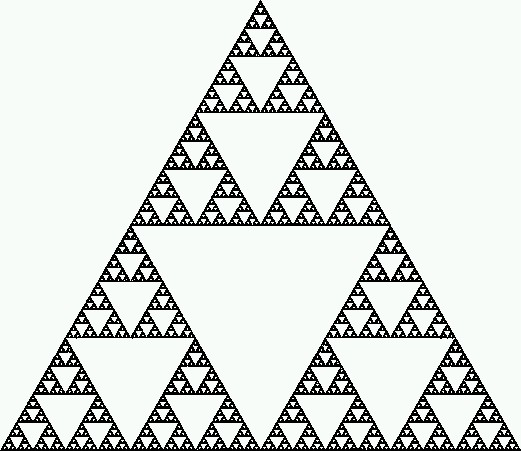
\includegraphics[width=0.5\textwidth]{sierpinski_triangle.jpg}
\end{figure}

The area of an equilateral triangle of side length $l$ is $\frac{\sqrt{3}}{4} l^2$, so that we have
\begin{equation*}
\Leb{2}(S) \le \Leb{2}(S_{k}) = 3^{k} \frac{\sqrt{3}}{4} 4^{-k}
\end{equation*}
for any $k \ge 0$. Therefore, by taking the limit as $k \to + \infty$, we conclude that $\Leb{2}(S) = 0$. We proceed now to estimate the Hausdorff measure of $S$. We notice that $$S_{k} = \bigcup_{j = 1}^{3^{k}} S_{k, j},$$ if we denote by $S_{k, j}$ the $j$-th equilateral triangle of the $k$-th iteration step. It is not difficult to see that $\diam(S_{k, j}) = 2^{-k}$. Therefore, since clearly $S \subset S_{k}$, for any $k \ge 0$, we see that, by choosing $\delta = 2^{-k}$, we obtain the following estimate
\[
\Haus{\alpha}_{\frac{1}{2^k}}(S) 
\leq \sum_{j=1}^{3^k}
\frac{\omega_\alpha}{2^\alpha} 
\left(\diam S_{k,j} \right)^\alpha 
= \frac{\omega_\alpha}{2^\alpha} 3^k 2^{-k\alpha},
%\searrow 0 \quad as \quad k\to \infty \quad \text{iff} \quad \alpha >
%\frac{\log^3}{\log^2}.
\]
which goes to zero for $k\to \infty$ if $\alpha >
\frac{\log^3}{\log^2}$. Thus, we can conclude that, for all $\alpha > \frac{\log{3}}{\log{2}}$, we
have $\Haus{\alpha}(S) = 0$, and this yields an upper bound on the Hausdorff dimension of $S$:
\[
\dim_{\mathcal{H}}(S) \leq \frac{\log 3}{\log 2}.
\]

\begin{figure}[!ht]
\caption{Sierpinski triangle decoration in a church}
\centering
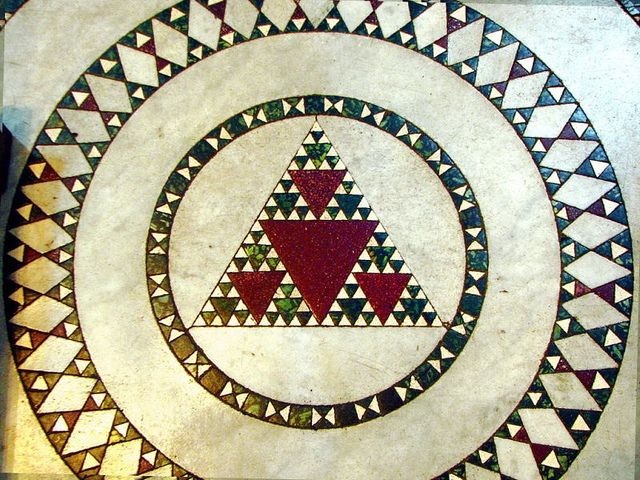
\includegraphics[width=0.3\textwidth]{sierpinski_triangle_decoration.jpg}
\end{figure}
\end{example}

We come now to the proof of Theorem \ref{thm:equivalence_Haus_Leb}, which is crucially based on the two following statements.

\begin{lemma}[Vitali covering property for $\Leb{n}$]
\label{lemmaVitaliCovering}
For all open $U$ and for all $\delta > 0$ there exists a family of disjoint
closed balls $\{\overline{B_k}\}_{k=1}^\infty$ such that $\diam B_k < \delta$ and
$\Leb{n}(U \setminus \bigcup_{k=1}^\infty \overline{B_k}) = 0$.
\end{lemma}

\begin{theorem}[Isodiametric inequality]
\label{thmIso}
For all $\Leb{n}$-measurable sets $E \subset \R^n$ we have 
\[
|E| \leq \omega_n \left(\frac{\diam E}{2}\right)^n.
\]
\end{theorem}

\begin{proof}[Proof of theorem \ref{thm:equivalence_Haus_Leb}]
The proof consists of three steps.~
\begin{enumerate}[({Step} 1) {Claim}:]
\item $\Leb{n}(A) \leq \Haus{n}_{\delta}(A)$ for all $A \subset \R^n$ and for all $\delta > 0$.
\\
Fix $\delta > 0$. Let $\{C_j\}_{j\in I}$: $A \subset \bigcup_{j\in I} C_j$, $\diam
C_j \leq \delta$. By the $\sigma$-subadditivity of the Lebesgue measure, we have
\[
\Leb{n}(A) \leq \sum_{j=1}^\infty \Leb{n}(C_j) \leq
\sum_{j=1}^\infty \omega_n \left(\frac{\diam C_j}{2}\right)^n,
\]
where in the last inequality we used the \emph{isometric
inequality}, Theorem \ref{thmIso}. Taking the
infimum over all such $\delta$-coverings $\{C_j\}_{j \in J}$, we obtain the claim
\[
\Leb{n}(A) \leq \Haus{n}_\delta (A) \qquad \text{for all} \quad
\delta > 0.
\]
%%% Step 2
\item for all $\delta > 0$, there exists $C_{n} \geq 1$ such that $\Haus{n}_{\delta} \leq C_n \Leb{n}$.

Notice that for any cube $Q$ we have
\begin{equation*}
\Leb{n}(Q) = \left(\frac{ \diam Q}{\sqrt{n}}\right)^n.
\end{equation*}
By the definition of the Lebesgue measure we get
\[
\begin{aligned}
\Leb{n}(A) 
&= \inf\left\{ \sum_{j=1}^\infty \Leb{n}(Q_j) \mid A
\subset \bigcup Q_j\right\}
\\& = \inf\left\{ \sum_{j=1}^\infty \Leb{n}(Q_j) \mid A
\subset \bigcup Q_j,\, \diam Q_j \le \delta \right\}
\\& = \frac{2^n}{\left(\sqrt{n}\right)^n \omega_n} \inf
\left\{\sum_{j=1}^\infty \omega_n \left(\frac{\diam Q_j}{2}\right)^n \mid 
A \subset \bigcup Q_j,\, \diam Q_j < \delta\right\}
\\&\geq \frac{1}{C_n} \Haus{n}_\delta (A),
\end{aligned}
\]
where in the second equality we used the fact that 
\[
\Leb{n} = \underbrace{\Leb{1} \times \dots \times \Leb{1}}_{n-\text{times}}\,,
\quad \text{and} \quad
\Leb{1} = \Haus{1}_\delta \quad \text{in } \R \quad \text{ for all } \delta > 0.
\]

\item $\Haus{n}_\delta(A) \leq \Leb{n}(A) + \varepsilon$ for any $\varepsilon >
0$.
\\
By the definition of $\Leb{n}$ we see that, for all fixed $\delta, \varepsilon > 0$, 
there exists a family $\{Q_j\}_{j=1}^\infty$ such that $A \subset
\bigcup_{j=1}^\infty Q_j$, $\diam Q_j \leq \delta$ 
and $\sum_{j=1}^\infty \Leb{n}(Q_j) \leq \Leb{n}(A) + \varepsilon$.
Now, by Lemma \ref{lemmaVitaliCovering}, there exists a family
$(\overline{B_j^i})_{i=1}^\infty$ of disjoint
closed balls such that $\overline{B_j^i} \subset Q_j$ for all $(\diam B^i_j \leq
\delta)$ and 
\vspace{-0.4em}
\[
%\vspace{-1em}
\Leb{n}\left(Q_j \setminus \bigcup_{i=1}^\infty
\overline{B_j^i}\right) = \Leb{n}\left(\overset{\circ}{Q}_j \setminus \bigcup_{i=1}^\infty
\overline{B_j^i}\right) 
= 0.
\]
Therefore, by Step 2 we also have
\vspace{-0.4em}
\[
\Haus{n}_\delta\left(Q_j \setminus \bigcup_{i=1}^\infty
\overline{B_j^i}\right) = 0,
\]
from which we deduce that
\[
\begin{aligned}
\Haus{n}_\delta(A) 
&\leq \sum_{j=1}^\infty \Haus{n}_\delta(Q_j) 
= \sum_{j=1}^\infty \Haus{n}_\delta \left(\bigcup_{i=1}^\infty
\overline{B_j^i}\right)
\\&= \sum_{j=1}^\infty  \sum_{i=1}^\infty
\Haus{n}_\delta \left( B_j^i\right)
\leq \sum_{j=1}^\infty  \sum_{i=1}^\infty
\underbrace{
\omega_n\left(\frac{\diam
B^i_j}{2}\right)^n}%
_{=\Leb{n}\left(\overline{B^i_j}\right)}
\\&= 
\sum_{j=1}^\infty  
\Leb{n}\left(\bigcup_{i=1}^\infty\overline{B^i_j}\right)
= 
\sum_{j=1}^\infty  
\Leb{n}(Q_j)
\\ &\leq \Leb{n}(A) + \varepsilon.
\end{aligned}
\]
\end{enumerate}
Since $\varepsilon > 0$ is arbitrary, this inequality ends the proof.
\end{proof}

\begin{proof}[Proof of the isodiametric inequality (Theorem \ref{thmIso})]
Without loss of generality, we may assume $E$ to be compact. Indeed, notice that $\diam A = \diam \overline{A}$ for any set $A$, and, if $\diam E = + \infty$, the inequality is trivially true.

Next, observe that, if $E \subset B\left (x, \frac{\diam E}{2}\right)$ for some $x \in \R^{n}$, then there is nothing to prove. We employ Steiner symmetrization\footnote{Introduced in 1838 by Jakob Steiner (1796 - 1863) \cite{steiner1838einfache}.} in order to reduce ourselves to such a case.

Decompose $\R^n = \R^{n-1}\times \R^1$ and let $p
: \R^n \to \R^{n-1}$, $q: \R^n \to \R$ be the orthogonal projections, $$p(x) = (x_{1}, \dots, x_{n - 1}), \quad q(x) =x_{n},$$ so that $$x = (p(x), q(x)) \quad \text{and} \quad |x|^2 = |p(x)|^2 + |q(x)|^2.$$ T
hen, for any $z \in \R^{n - 1}$ we define the {\em verital section}
\[
 E_z := \left\{t\in\R : (z,t) \in E\right\},
\]
and, as a consequence, we introduce the {\em symmetrization} of $E$ with respect $n$-th coordinate axis:
\[
E^s := \left\{ x \in \R^n: |q(x)| \leq \frac{\Leb{1}(E_{p(x)})}{2}\right\}.
\]
By Fubini's theorem, $E_z$ is $\Leb{1}$-measurable for
$\Leb{n-1}$-a.e. $z$, $z \mapsto \Leb{1}(E_z)$ is Lebesgue
measurable and so we get
\begin{equation} \label{eq:Lebesgue_symm_equality}
|E| = \int_{\R^{n-1}} \Leb{1}(E_z) dz = \int_{\R^{n-1}}
\Leb{1}(E_z^s) dz = |E^s|,
\end{equation}
where the first equality follows by Fubini's theorem, and the second one is a consequence of the fact that
\[
(E^s)_z = \{ t\in\R : (z,t) \in E^s \}
= \left\{ t\in \R : |t| \leq \frac{\Leb{1}(E_z)}{2} \right\}
= \left[ - \frac{\Leb{1}(E_z)}{2}, \frac{\Leb{1}(E_z)}{2} \right].
\]

Now we claim that
\begin{equation} \label{eq:diam_control}
\diam E^s \leq \diam E.
\end{equation}
In order to prove this, let $x \in E^s$ and define $M(x), m(x)
\in E$ to be the points for which 
\[
\begin{aligned}
p(m(x)) &= p(M(x)) = p(x)
\\
q(m(x)) &\le q(z) \leq q(M(x))
\qquad \text{for all} \quad z \in E \quad \text{with} \quad p(z) = p(x).
\end{aligned}
\]
Hence, for all $x,y \in E^s$, we have
\[
|q(x) - q(y)| \leq \max \left\{|q(M(x)) - q(m(y))|, |q(M(y)) - q(m(x))|\right\},
\]
in particular, without loss of generality, we can assume that
$$\max \left\{|q(M(x)) - q(m(y))|, |q(M(y)) - q(m(x))|\right\} = |q(M(x)) - q(m(y))|,$$
so that
$$ |q(x) - q(y)| \leq |q(M(x)) - q(m(y))|.$$
As a consequence, we see that
\begin{align*}
|x-y|^2 & = |p(x-y)|^2 + |q(x-y)|^2 \leq |p(M(x)) - p(m(y))|^2 + |q(M(x)) - q(m(y))|^2 \\
& = |M(x) - m(y)|^2 = \max \left\{|M(x) - m(y)|, |M(y) - m(x)|\right\}^2 \leq (\diam E)^2 .
\end{align*}
This means that $|x - y| \leq \diam E$ for all $x,y \in E^s$, which immediately implies \eqref{eq:diam_control}.

Given a $\Leb{n}$ measurable set $F$, we define $F^i$ to be the Steiner
symmetrization with respect to the $i$-th coordinate axis. Hence, if we set $E_0 := E$, $E_i := (E_{i=1})^i$ with $i \in \{1,2,\dots,n\}$, then, by \eqref{eq:Lebesgue_symm_equality} we have $|E_n| = |E|$ and $\diam E_n \leq \diam E$ by \eqref{eq:diam_control}. In addition, we notice that, if $x\in E_n$, then $-x \in E_n$, which implies $E_n \subset B\left(0,\frac{\diam E_n}{2}\right)$. Thus, we conclude that
\begin{equation*}
|E| = |E_{n}| \le \omega_{n} \left ( \frac{\diam E_{n}}{2} \right )^{n} \le \omega_{n} \left ( \frac{\diam E}{2} \right )^{n}.
\end{equation*}
And so we are done!
\end{proof}

\section{Integration and fundamental convergence theorems}
 
In this section, let $X \neq \emptyset$, and $\mu$ be a measure on $X$. Recall the definition of the {\em extended real line} $$\overline{\R}:= [-\infty,\infty].$$

\begin{definition}~
\begin{enumerate}[(1)]
\item A function $u : X \to \overline{\R}$ is \emph{$\mu$-measurable} if the {\em superlevel set} $$\{u > t\} := \{ x \in X : u(x) > t\}$$ 
is $\mu$-measurable for all $t\in \overline{\R}$.
\item A function $u : X \to \overline{\R}$ is a \emph{$\mu$-simple function} if it is $\mu$-measurable and $u(X)$ is
countable; that is, $$u(x) = \sum_{k=1}^\infty u_k \chi_{E_k}(x),$$
for some sequences of real numbers $\{u_{k}\}$ and of $\mu$-measurable disjoint sets $\{E_{k}\}$.
\item If $u$ is a nonnegative $\mu$-simple function, we define 
\[
\int_X u \, d\mu := \sum_{t \in u(X)} t\mu(\{u=t\}) = \sum_{k=1}^\infty u_k
\mu(E_k) \in [0,\infty]
\]
with the convention that $0 \cdot \infty = 0$.
\item We set $u^\pm := \max\{\pm u, 0 \}$, so that $u = u^+ - u^-$ and $|u| = u^{+} + u^{-}$. 
If $u$ is $\mu$-simple and $\int_X u^+ d\mu$ or $\int_X u^- d\mu < \infty$, then $u$ is a {\em $\mu$-integrable simple function}, and we set
\begin{equation*} 
\int_X u \, d\mu := \int_X u^+ d\mu - \int_X u^- d\mu \in [-\infty,\infty]
\end{equation*}
\item If $u : X \to \overline{\R}$ is $\mu$-measurable, we define the {\em upper and lower integrals} of $u$
as
\[
\int^*_X u \, d\mu := \inf \left\{ \int_X v \, d\mu \mid 
\text{$v \geq u$ $\mu$-a.e, $v$ $\mu$-integrable simple function}
\right\}
\]
or
\[
%{\phantom{\int}}_{*}\hspace{-0.3em}\int_{X} 
\int_{* X} u \, d\mu := \sup\left\{ \int_X v \, d\mu \mid 
\text{$v \leq u$ $\mu$-a.e, $v$ $\mu$-integrable simple function}
\right\}
\]
respectively. 
If
\[
\int_{* X} u \, d\mu = \int^*_X u \, d\mu,
\]
then we say that $u$ is {\em $\mu$-integrable}, and we set
\begin{equation*}
\int_{X} u \, d \mu := \int^*_X u \, d\mu = \int_{* X} u \, d\mu.
\end{equation*}
\item A measurable function $u$ is \emph{$\mu$-summable} if $|u|$ is
$\mu$-integrable and 
\[
\int_X |u| \, d\mu < \infty.
\]
\end{enumerate}
\end{definition}

\begin{example}[Integral with respect to the Dirac measure] \label{example_delta_measure_int}
Let $x_{0} \in X$ and $\mu = \delta_{x_{0}}$ be the Dirac measure centered in $x_{0}$, as defined in Example \ref{example_delta_measure}. Notice that any subset in $X$ is $\delta_{x_{0}}$-measurable, so that any function $u: X \to \overline{\R}$ is $\delta_{x_{0}}$-measurable. Then, any $u : X \to \overline{\R}$ simple function is $\mu$-integrable. Indeed, assuming at first $u : X \to [0, \infty]$, for some sequence of nonnegative real numbers $\{u_{k}\}$ and a partition $\{E_{k}\}$ of $X$, we have
\begin{equation*}
u(x) = \sum_{k=1}^\infty u_k \chi_{E_k}(x),
\end{equation*}
so that
\begin{equation*}
\int_{X} u \, d \delta_{x_{0}} = \sum_{k = 1}^{\infty} u_{k} \delta_{x_{0}}(E_{k}) = u_{k_{0}},
\end{equation*}
where $k_{0}$ satisfies $E_{k_{0}} \ni x_{0}$, which implies $u(x_{0}) = u_{k_{0}}$. Then, if $u : X \to \overline{\R}$ is simple, then we have either $u^{+}(x_{0}) > 0$ or $u^{-}(x_{0}) > 0$, so that either 
\begin{equation*}
\int_{X} u^{-} \, d \delta_{x_{0}} = 0 \quad \text{or} \quad \int_{X} u^{+} \, d \delta_{x_{0}}  = 0,
\end{equation*}
respectively.
Therefore, we can easily see that
\begin{equation*}
\int_{X} u \, d \delta_{x_{0}} = u^{+}(x_{0}) - u^{-}(x_{0}) = u(x_{0})
\end{equation*}
for any simple function $u$. As a consequence, any $u : X \to \overline{\R}$ is $\delta_{x_{0}}$-integrable. Indeed, for any simple function $v \ge u$ and any simple function $w \le u$, we have
\begin{equation*}
w(x_{0}) \le \int_{* X} u \, d\delta_{x_{0}} \le \int^*_X u \, d\delta_{x_{0}} \le v(x_{0}),
\end{equation*} 
so that we get 
\begin{equation*}
\int_{* X} u \, d\delta_{x_{0}} = \int^*_X u \, d\delta_{x_{0}} = u(x_{0}),
\end{equation*}
by choosing 
\begin{equation*}
v(x) = \begin{cases} u(x_{0}) & x = x_{0}, \\
+ \infty & x \neq x_{0},
\end{cases}
\end{equation*}
and
\begin{equation*}
w(x) = \begin{cases} u(x_{0}) & x = x_{0}, \\
- \infty & x \neq x_{0}.
\end{cases}
\end{equation*}
Thus, we conclude that, for any $u: X \to \overline{\R}$, we have
\begin{equation*}
\int_{X} u \, d \delta_{x_{0}} = u(x_{0}),
\end{equation*}
and that $u$ is $\delta_{x_{0}}$-summable if and only if $|u(x_{0})| < \infty$. 
\end{example}

%On the other hand, $u(x_{0}) = + \infty$, then any simple function $v \ge u$ satisfies $v(x_{0}) = + \infty$, so that
%\begin{equation*}
%\int^*_X u \, d\delta_{x_{0}} = +\infty,
%\end{equation*}
%while we can choose a sequence of simple functions $v \le u$ satisfying $v(x_{0}) = k$, for any $k \in \N$, so that
%\begin{equation*}
%{\phantom{\int}}_{*}\hspace{-0.3em}\int_{X} u \, d\delta_{x_{0}} \ge k,
%\end{equation*}
%which implies that also the lower integral must be $+ \infty$. Thus we have
%\begin{equation*}
%\int^*_X u \, d\delta_{x_{0}} = {\phantom{\int}}_{*}\hspace{-0.3em}\int_{X} u \, d\delta_{x_{0}} = + \infty,
%\end{equation*}
%and one can argue similarly in the case $u(x_{0}) = - \infty$.

We define now general versions of the familiar $L^{p}$-function spaces.

\begin{definition} \hfill
\begin{itemize}[]
\item $L^1(X,\mu) := \left\{ u: X \to \overline{\R} : \text{$u$ is
$\mu$-summable} \right\}$ and we set $$\|u\|_{L^{1}(X, \mu)} := \int_{X} |u| \, d \mu.$$
%\item $L_{\textnormal{loc}}^1(X,\mu) := \left\{ u: X \to \overline{\R} \mid \|u\chi_K \|_{L^{1}(X, \mu)} < \infty \text{ for all $K\subset X$ compact} \right\}.$
\item For any $p \in (1, \infty)$, we define $L^p(X,\mu) := \left\{ u: X \to \overline{\R} : \text{$|u|^p$ is
$\mu$-summable} \right\}$ and we set $$\|u\|_{L^{p}(X, \mu)} := \left ( \int_{X} |u|^p \, d \mu \right )^{\frac{1}{p}}.$$
%\item $L_{\textnormal{loc}}^{p}(X,\mu) := \left\{ u: X \to \overline{\R} \mid \|u\chi_K \|_{L^{p}(X, \mu)} < \infty \text{ for all $K\subset X$ compact} \right\}.$
\item Let $u : X \to \overline{R}$ be $\mu$-measurable. We set $$\|u\|_{L^{\infty}(X, \mu)} := \inf \left \{ \lambda > 0 : \mu(\{ |u| > \lambda \}) = 0 \right \}.$$
As a consequence, we define $L^{\infty}(X, \mu) := \left \{ u: X \to \overline{\R} :  \|u\|_{L^{\infty}(X, \mu)} < \infty \right \}$.
\item For any $p \in [1, \infty]$, we define the local $L^{p}$-spaces as
$$L^{p}_{\rm loc}(X,\mu) := \left\{ u: X \to \overline{\R} : \|u\chi_K \|_{L^{p}(X, \mu)} < \infty \text{ for all $K\subset X$ compact} \right\}.$$
\end{itemize}
\item For any $m \in \N$, we set $L^{p}(X, \mu; \R^{m}) := \left \{ u: X \to \R^{m} : |u| \in L^{p}(X, \mu) \right \}$, with
$$ \|u\|_{L^{p}(X, \mu; \R^{m})} := \||u|\|_{L^{p}(X, \mu)}, \quad |u(x)| := \sqrt{\sum_{j = 1}^{m} u_{j}(x)^{2}},$$
and 
$$L^{p}_{\rm loc}(X, \mu; \R^{m}) := \left \{ u : X \to \R^{m} : \|u\chi_K \|_{L^{p}(X, \mu; \R^{m})} < \infty \text{ for all $K\subset X$ compact} \right\}.$$
\end{definition}

In the case $X = \R^{n}$ and $\mu = \Leb{n}$, we shall set for brevity 
\begin{equation*}
L^{p}(\R^{n}; \R^{m}) := L^{p}(\R^{n}, \Leb{n}; \R^{m}) \quad \text{and} \quad L^{p}_{\rm loc}(\R^{n}; \R^{m}) := L^{p}_{\rm loc}(\R^{n}, \Leb{n}; \R^{m}),
\end{equation*} 
for any $p \in [1, \infty]$.

\begin{example}[The spaces $L^{p}(X, \delta_{x_{0}})$]
In light of Example \ref{example_delta_measure_int}, we see that, for all $x_{0} \in X$ and $p \in [1, \infty]$, the spaces $L^{p}(X, \delta_{x_{0}})$ and $L^{p}_{\rm loc}(X, \delta_{x_{0}})$ all coincide with the space
\begin{equation*}
\left \{ u : X \to \overline{\R} : |u(x_{0})| < + \infty \right \}.
\end{equation*}
\end{example}

We recall now the simple and very useful Chebychev inequality.

\begin{proposition}[Chebychev inequality] \label{prop:Cheb_ineq}
Let $u : X \to [0, + \infty]$ be $\mu$-integrable. Then, for all $t > 0$, we have
\begin{equation} \label{eq:Cheb_ineq}
\int_{\{u \ge t\}} u \, d \mu \ge t \mu(\{ u \ge t \}).
\end{equation}
\end{proposition}
\begin{proof}
If $u$ is simple, then we have
\begin{equation*}
u(x) = \sum_{k = 1}^{\infty} u_{k} \chi_{E_{k}}(x),
\end{equation*}
and so
\begin{equation*}
\int_{\{u \ge t\}} u \, d \mu = \int_{X} u \chi_{\{u \ge t\}} \, d \mu \ge t \sum_{k : u_{k} \ge t} \mu(E_{k} \cap \{ u \ge t \}) = t \mu(\{ u \ge t \}).
\end{equation*}
Then the conclusion follows by approximation with simple functions.
\end{proof}

\begin{remark} \label{rem_easy_Cheb} Let $u : X \to \overline{\R}$ be a $\mu$-integrable function. Then, we have the following simple consequence of the Chebychev inequality (Proposition \ref{prop:Cheb_ineq}):
\begin{enumerate}[i)]
\item if $\int_{X} |u| \, d \mu < + \infty$, then $\mu(\{ |u| = + \infty\}) = 0$;
\item if $\int_{X} |u| \, d \mu = 0$, then $u(x) = 0$ for $\mu$-a.e. $x \in X$. 
\end{enumerate}
It is easy to see that (i) follows from \eqref{eq:Cheb_ineq}, since
\begin{equation*}
\int_{X} |u| \, d \mu \ge \int_{\{|u| = + \infty\}} |u| \, d \mu = \int_{\{|u| = + \infty\} \cap \{|u| \ge t\}} |u| \, d \mu \ge t \mu(\{ |u| = + \infty\}) 
\end{equation*}
for all $t > 0$, since $\{|u| = + \infty\} \cap \{|u| \ge t\} = \{|u| = + \infty\}$.
Instead, in order to prove (ii), it is enough to notice that, again by \eqref{eq:Cheb_ineq}, for any $\eps > 0$ we have
\begin{equation*}
0 = \int_{X} |u| \, d \mu \ge \int_{\{|u| \ge \eps\}}|u| \, d \mu \ge \eps \mu(\{ |u| \ge \eps \}),
\end{equation*} 
so that 
\begin{equation*}
\mu\left(\{ |u| > 0\}\right) = \mu \left ( \bigcup_{k = 1}^{\infty} \left \{ |u| \ge \frac{1}{k} \right \} \right ) \le \sum_{k = 1}^{\infty} \mu \left ( \left \{ |u| \ge \frac{1}{k} \right \} \right ) = 0.
\end{equation*}
\end{remark}

We recall now some fundamental convergence results concerning the exchange between limits and integrals.

\begin{theorem}[Monotone convergence theorem] \label{thm:monotone_thm}
If $\{u_{k}\}_{k \in \N}$ is a sequence of nonnegative $\mu$-measurable functions such that $u_{k} \le u_{k + 1}$ $\mu$-a.e. on $X$ for all $k \in \N$, then
\begin{equation*}
\lim_{k \to + \infty} \int_{X} u_{k} \, d \mu = \int_{X} \sup_{k \in \N} u_{k} \, d\mu.
\end{equation*}
If instead $u_{k} \ge u_{k + 1}$ $\mu$-a.e. on $X$ for all $k \in \N$ and $u_{1} \in L^{1}(X, \mu)$, then
\begin{equation*}
\lim_{k \to + \infty} \int_{X} u_{k} \, d \mu = \int_{X} \inf_{k \in \N} u_{k} \, d\mu.
\end{equation*}
\end{theorem}

\begin{theorem}[Fatou's lemma] \label{thm:Fatou}
If $\{u_{k}\}_{k \in \N}$ is a sequence of nonnegative $\mu$-measurable functions, then
\begin{equation*}
\int_{X} \liminf_{k \to + \infty} u_{k} \, d \mu \le \liminf_{k \to + \infty} \int_{X} u_{k} \, d \mu.
\end{equation*}
\end{theorem}

\begin{theorem}[Dominated convergence theorem] \label{thm:dominated_convergence}
Let $\{u_{k}\}_{k \in \N}$ be a sequence of $\mu$-measurable functions such that there exist a $\mu$-measurable function $u$ satisfying $u_{k}(x) \to u(x)$ for $\mu$-a.e. $x \in X$ and $v \in L^{1}(X, \mu)$ satisfying $|u_{k}| \le v$ $\mu$-a.e. on $X$ for all $k \in \N$. Then, we have
\begin{equation*}
\lim_{k \to + \infty} \int_{X} |u_{k} - u| \, d \mu = 0,
\end{equation*}
and, in particular,
\begin{equation*}
\lim_{k \to + \infty} \int_{X} u_{k} \, d \mu = \int_{X} u \, d \mu.
\end{equation*}
\end{theorem}

\begin{theorem}
Assume $u_{k}, u$ are $\mu$-summable functions, for all $k \in \N$, and
\begin{equation*}
\lim_{k \to + \infty} \int_{X} |u_{k} - u| \, d \mu = 0.
\end{equation*}
Then there exists a subsequence $\{u_{k_{j}}\}$ such that $u_{k_{j}}(x) \to u(x)$ for $\mu$-a.e. $x \in X$.
\end{theorem}
\begin{proof}
Let $\{u_{k_{j}}\}$ be a subsequence satisfying
\begin{equation*}
\sum_{j = 1}^{\infty} \int_{X} |u_{k_{j}} - u| \, d \mu < \infty.
\end{equation*}
Notice that such a subsequence exists, since 
\begin{equation*}
a_{k} := \int_{X} |u_{k} - u| \, d \mu  \to 0,
\end{equation*}
so that we can select a subsequence $a_{k_{j}}$ satisfying $a_{k_{j}} \le 2^{-j}$ for all $j \in \N$. By the monotone convergence theorem (Theorem \ref{thm:monotone_thm}), we have
\begin{equation*}
\sum_{j = 1}^{\infty} \int_{X} |u_{k_{j}} - u| \, d \mu = \int_{X} \sum_{j = 1}^{\infty} |u_{k_{j}} - u| \, d \mu < \infty.
\end{equation*}
Therefore, by Remark \ref{rem_easy_Cheb}, we obtain 
\begin{equation*}
\sum_{j = 1}^{\infty} |u_{k_{j}}(x) - u(x)| < \infty
\end{equation*}
for $\mu$-a.e. $x \in X$, and thus we conclude that $u_{k_{j}}(x) \to u(x)$ for $\mu$-a.e. $x \in X$.
\end{proof}

Thanks to the notion of integral with respect to a general measure $\mu$, it is plain to see that the integration of a nonnegative $\mu$-measurable function is itself a measure, so that we can formulate the following definition.

\begin{definition}[Integral measures] \label{def:intregral_measure}
If $u : X \to [0,\infty]$ $\mu$-measurable, then we define the {\em integral measure} $\nu = u \mu$ (or
$\mu \res u$) as 
\[
\nu(A) = \int_A u \, d\mu = \int_X u \chi_A \, d\mu 
\qquad \text{for all } \mu\text{-measurable } A.
\]
\end{definition}

\section{Real and vector valued Radon measures}

Through this section, let $\Omega \subset \R^{n}$ be an open set. We exploit now the concept of integral measure introduced in Definition \ref{def:intregral_measure} to define signed and vector valued Radon measures. In order to avoid ambiguity, from this point on we shall refer to the Radon measure introduced in Definition \ref{def:Borel_Radon_measure} as nonnegative Radon measures.

\begin{definition}[Signed Radon measures]
Given a nonnegative Radon measure $\mu$ on $\Omega$ and $f: \Omega \to
[-\infty,\infty]$ locally $\mu$-summable. Then we set $\nu := f \mu$ to be the integral measure satisfying
\[
\nu(K) = \int_K f \, d\mu 
\qquad \text{for all }  K \, \text{compact.}
\]
$\nu$ is said to be a \emph{signed Radon measure} on $\Omega$.
\end{definition}

\begin{definition}[Vector valued Radon measures]
Given a nonnegative Radon measure $\mu$ on $\Omega$ and $f: \Omega \to
\R^m$ is locally $\mu$-summable. Then we set $\nu := f \mu$ to be the vector valued Radon measure satisfying
\[
\nu(K) = \int_K f \, d\mu 
\qquad \text{for all }  K \, \text{compact.}
\]
$\nu$ is said to be a \emph{vector valued Radon measure} on $\Omega$.
\end{definition}

Exploiting the inner regularity of the 


\begin{definition}[Alternative approach] \hfill
\begin{itemize}
\item A nonnegative Radon measure is a mapping $\mu : \mathcal{B}(\Omega) \to
[0,\infty]$ which is $\sigma$-additive and finite on compact sets. We denote the space of such measures by $\mathcal{M}_{\rm loc}^{+}(\Omega)$.
\item A vector valued (real or signed if $m = 1$) Radon measure is a mapping $\mu :
\mathcal{B}(\Omega) \to \R^m$ which is $\sigma$-additive and its total variation
$|\mu|$ is finite on compact sets; that is
\[
|\mu|(K) := \sup \left\{
\sum_{j=1}^\infty |\mu(B_j)| \mid K = \bigcup_{j} B_j, B_i \cap B_i = \emptyset
\text{ if } i\neq j
\right\} < \infty \text{ for all $K$ compact in $\Omega$}.
\]
The space of such measures is denote by $\mathcal{M}_{\rm loc}(\Omega; \R^{m})$; and by $\mathcal{M}_{\rm loc}(\Omega)$ if $m = 1$.
\item We say that a nonnegative Radon measure $\mu : \mathcal{B}(\Omega) \to
[0,\infty)$ is finite if $\mu(\Omega) < \infty$; and we denote by $\mathcal{M}^+(\Omega)$ the space of such measures.
\item We say that a nonnegative vector-valued Radon measure $\mu : \mathcal{B}(\Omega) \to
\R^m$ is finite if $|\mu|(\Omega) < \infty$; and we denote by $\mathcal{M}(\Omega,\R^m)$, and $\mathcal{M}(\Omega)$ if $m = 1$, the space of such measures.
\end{itemize}
\end{definition}

\begin{remarks}[Basic facts] \hfill
\begin{itemize}
\item If $\mu \in \mathcal{M}_{loc}(\Omega,\R^m)$, then $|\mu| \in
\mathcal{M}^+_{loc}(\Omega)$, where
\[
|\mu|(B) := \sup \left \{\sum_{j=1} ^\infty |\mu(B_j)| \mid 
B= \bigcup B_j, B_j \cap B_i = \emptyset \, i\neq j, B_j \in \mathcal{B}(\Omega)
\right \}
\]
for any $B \Subset \Omega$.
In particular, $\sum \mu(B_j)$ is absolutely convergent for all $\{B_j\}$
partition of a some set $B \Subset \Omega$.
\item The total variation is the smallest nonnegative Radon measure $\nu$ such
that $\nu (B) \geq |\mu(B)|$ for all $B \in \mathcal{B}(\Omega)$.
\item If $\mu \in \mathcal{M}(\Omega)$, we define the {\em positive and negative
parts} of $\mu$ 
\[
\mu^+ := \frac{|\mu| + \mu}{2} \quad \text{and} \quad
\mu^- := \frac{|\mu| - \mu}{2}.
\]
It is easy to notice that $\mu^{\pm} \geq 0$ and that $\mu = \mu^{+} - \mu^{-}$, which is the {\em Jordan decomposition}, and it is unique. In addition, $|\mu| = \mu^{+} + \mu^{-}$.
\end{itemize}
\end{remarks}

\begin{lemma}
If $\mu \in \mathcal{M}^+(\Omega)$ and $f\in L^1(\Omega,\mu;\R^m)$, then $f\mu \in \mathcal{M}(\Omega,\R^m)$ and $|f\mu| = |f|\mu$.
\end{lemma}
\begin{proof}
Let $B \in \mathcal{B}(\Omega)$.
\begin{itemize}
\item It is easy to notice that
\begin{equation*}
|(f \mu)(B)| := | \int_B f d\mu| \leq \int_B |f| d\mu.
\end{equation*} 
From this it follows immediately that $|f\mu| \leq |f| \mu$, which implies $f\mu \in \mathcal{M}(\Omega;\R^m)$. 
\item Let $\varepsilon > 0$ and $D = \{z_h\}_{h\in\N}$ countable dense set in
$\S^{m-1}$, let $B \in \mathcal{B}(\Omega)$. We define 
\[
\sigma(x) := \min \{h\in \N: f(x) z_h \geq (1-\varepsilon)|f(x)|\}
\]
it is Borel measurable. Then, we set $$B_h : = \sigma^{-1}(\{h\}) \cap B,$$ 
and we notice that 
\begin{equation*}
B_{h} \in \mathcal{B}(\Omega), \ B = \bigcup_{h\in\N} B_h \text{ and } B_h \cap B_k = \empty \text{ if } h\neq k. 
\end{equation*}
This implies that 
\[
\begin{aligned}
\int_B |f| d\mu 
&= \sum_{k\in\N} \int_{B_h} |f| d\mu 
\leq \frac{1}{1-\varepsilon} \sum_{h\in\N} \int_{B_h} f z_h d\mu 
\leq \frac{1}{1-\varepsilon} \sum_{h\in\N} |(f \mu)(B_h)|  
\leq \frac{1}{1-\varepsilon}  |f \mu|(B),
\end{aligned}
\]
since 
\[
\int_{B_h} f z_h d\mu 
= z_h \int_{B_h} f d\mu 
\leq \left|\int_{B_h} f d\mu \right|
= |(f \mu)(B_h)|  
\]
\end{itemize}
\end{proof}

\begin{definition}
Let $\mu$ be a nonnegative measure on $\Omega$.
\begin{itemize}
\item We say that $\mu$ is concentrated on a set $E \subset \Omega$ if  
\[
\mu(\Omega \setminus E) = 0.
\]
\item We call the support of $\mu$, $\supp \mu$, the smallest closed set on
which $\mu$ is concentrated :
\[
\supp (\mu) := \bigcap_{C \text{ closed}, \mu (\Omega\setminus C) = 0} C.
\]
\end{itemize}
\end{definition}

\begin{exercise}
Equivalently, we may characterize the support of a nonnegative Radon measure $\mu$ in terms of its behaviour on balls:
\[
\supp (\mu) = \{x \in \Omega \mid \mu(B(x,r)) > 0, \forall r > 0 \, \text{ such that } B(x,r) \subset \Omega\}
\]
\end{exercise}

\begin{remark}
Notice that a nonnegative Radon measure may be concentrated on a set strictly smaller than its support. Indeed, let $\Omega = \R$ and $$\mu = \sum_{k = 1}^{\infty} \frac{1}{2^{k}} \delta_{\frac{1}{k}}.$$
It is clear that $\mu$ is concentrated on the set $E = \left \{ \frac{1}{k}\right \}_{k \ge 1}$, but $\mu((-r, r)) > 0$ for any $r> 0$, so that $0 \in \supp(\mu)$. In fact, it is not difficult to check that $\supp(\mu) = \{0\} \cup \left \{ \frac{1}{k}\right \}_{k \ge 1} = \overline{E}$. 
\end{remark}

\begin{definition}\hfill
\begin{enumerate}[1.]
\item Let $\mu \in \mathcal{M}^{+}_{\rm loc}(\Omega)$, $\nu \in \mathcal{M}_{\rm loc}(\Omega,\R^m)$. We say
that $\mu$ is absolutely continuous with respect to $\mu$, and we write $\nu \ll \mu$, if
for all $B \in \mathcal{B}(\Omega)$ such that $\mu(B) = 0$, then $|\nu|(B) = 0$.
\item If $\mu,\nu \in \mathcal{M}^+_{\rm loc}(\Omega)$, we say that they are mutually
singular if there exists $E,F \in \mathcal{B}(\Omega)$ such that $\mu(F) =0$,
$\mu(E) = 0$ and 
\[
\mu(B) = \mu (B\cap E) \qquad \text{and} \qquad
\nu(B) = \nu(B \cap F)
\]
for all $B \in \mathcal{B}(\Omega)$ and we write $\mu \perp \nu$. If $\mu,\nu
\in \mathcal{M}_{\rm loc}(\Omega,\R^m)$, 
\[
\mu \perp \nu \iff |\mu| \perp |\mu|
\]
\end{enumerate}
\end{definition}

\begin{theorem}[Radon-Nikodym] \label{thm:Radon_Nikodym}
Let $\mu \in \mathcal{M}(\Omega,\R^m)$, $\mu \in \mathcal{M}^+(\Omega)$. Then
there exist unique measures $\nu^{ac},\nu^{s} \in \mathcal{M}(\Omega; \R^m)$ such
that $\nu^{ac} \ll \mu$, $\nu^s \perp \mu$ and 
\begin{equation} \label{eq:Leb_decomp}
\nu = \nu^{ac} + \nu^s. 
\end{equation}
In addition, there exists a unique measure $f\in L^1(\Omega,\mu;\R^m)$ such that
$\nu^{ac} = f\mu$.
\\
In particular, if $\mu = \Leb{n}$, every $\mu \in \mathcal{M}(\Omega;\R^m)$ can be
uniquely decomposed in
\[
\mu = f \Leb{n} + \nu^s, 
\]
for some $f\in L^1(\Omega; \R^n)$ and $\nu^s \in \mathcal{M}(\Omega;\R^m), \nu^s \perp \Leb{n}$.
\end{theorem}

The decomposition in \eqref{eq:Leb_decomp} is called {\em Lebesgue decomposition} of the measure $\nu$ with respect to $\mu$.

\begin{definition} We say that a property holds $|\mu|$-almost everywhere or for
$|\mu|$-almost every $x$ if the set where the property does not hold is
$|\mu|$-negligible; that is, it has zero $|\mu|$-measure.
\end{definition}

\begin{corollary}[Polar decomposition]
Let $\mu \in \mathcal{M}(\Omega;\R^m)$. Then there exists a unique $f \in
L^1(\Omega,|\mu|;\R^m)$ such that $|f(x)| =1 $ $|\mu|$-a.e and $\mu = f|\mu|$.
\end{corollary}

\begin{proof}[Proof of corollary]
Apply Radon-Nikodym theorem (Theorem \ref{thm:Radon_Nikodym}) to $\mu$ and $|\mu|$. We know that 
\(
|\mu(B)| \leq |\mu|(B) 
\)
for all $B \in \mathcal{B}(\Omega)$. From this follows $\mu \ll |\mu|$, and so there exists $f \in L^{1}(\Omega, |\mu|; \R^{m})$ such that $\mu = f|\mu|$.
\\
We proved that $|f|\mu|| = |f||\mu|$, hence we obtain
\[
|\mu| = |f|\mu|| = |f||\mu|
\quad \text{and so} \quad
(|f| - 1)|\mu| = 0.
\]
This means that we have
\[
\int_{\Omega}(|f| - 1)d|\mu| = 0,
\]
which yields $|f(x)| =1$ for $|\mu|$-a.e. $x \in \Omega$. 
\end{proof}

\begin{corollary}[Hahn decomposition]
Let $\mu \in \mathcal{M}(\Omega)$, there exists a unique $A \in
\mathcal{B}(\Omega)$ (up to $|\mu|$-negligible sets) such that 
\[
\mu^+ = \mu \res A
\qquad 
\mu^- = -\mu \res (\Omega \setminus A).
\]
\end{corollary}
\begin{proof}
By the polar decomposition, there exists a unique $f \in L^{1}(\Omega, |\mu|)$ such that $\mu = f|\mu|$ and $f(x) \in \{\pm 1\}$ for
$|\mu|$-a.e. $x\in\Omega$. This means that, if we set
$$A:= \{f =1 \},$$
we have
\begin{equation*}
f(x) = \chi_A - \chi_{\Omega\setminus A}.
\end{equation*}
Thus, we obtain
\begin{align*}
\mu^+ & := \frac{|\mu| + \mu}{2} = \frac{ 1 + \chi_A - \chi_{\Omega\setminus A}}{2} |\mu| = \chi_{A} |\mu|, \\
\mu^- & := \frac{|\mu| - \mu}{2} = \frac{1 - \chi_{A} + \chi_{\Omega \setminus A}}{2} |\mu| = \chi_{\Omega \setminus A} |\mu|.
\end{align*}
\end{proof}

\section{Duality for Radon measures}

Another characterization is given via the duality with continuous functions.

\begin{definition}
We say that $B \Subset \Omega$ if $\overline{B} \subset \Omega$ and it is
compact in $\Omega$.
\[
C^0_C(\Omega; \R^m) := \{u \in C^0(\Omega;\R^m) : \supp u \Subset \Omega \}
\]
\[
C^0_0(\Omega; \R^m) := \{u \in C^0(\Omega;\R^m) : \forall \varepsilon > 0 \
\exists K \subset \Omega: |u(x)| < \varepsilon \quad \forall x \not\in K 
\}
\]
\[
\|u\|_{\infty} : = \sup_{x \in \Omega} |u(x)|
\]
\end{definition}

\begin{remark}
$C^0_0(\Omega;\R^m) = \overline{C^0_c(\Omega;\R^n)}^{\|\cdot\|_\infty}$,
$(C^0_0(\Omega;\R^n),\|\cdot\|_\infty)$ is Banach.
$C^0_c$ is separable, locally convex, topological vector space with the
following topology:
\[
\varphi_k \longrightarrow \varphi \quad \text{in} \quad C^0_c 
\quad \iff \quad
\|\varphi_k - \varphi\|_\infty \to 0
\quad \text{and there exists } K \subset \Omega:
\supp \varphi \cup \bigcup_{k\in\N} \supp \varphi_k \subset K
\]
\end{remark}

\begin{theorem}[Lusin]
Let $\mu$ Borel on $\Omega$ and $u : \Omega \to \R$ is $\mu$-measurable, $u
\equiv 0$ in $\Omega \setminus E$ with $\mu(E) < \infty$. Then for all
$\varepsilon > 0$ there exists $v \in C^0(\Omega)$ such that $\|v\|_\infty
\leq \|u\|_\infty$
\[
\mu(\{x \in \Omega: v(x) \neq u(x)\}) < \varepsilon.
\]
\end{theorem}

\begin{remark}
An equivalent formulation states that, under the additional assumption
$\mu(\Omega) < \infty$, then there exists a sequence of compact sets $\{K_h\}$ such that
\[
\mu \left (\Omega \setminus \bigcup_{h = 1}^{\infty} K_h \right ) = 0
\qquad \text{and} \qquad
u\big|_{K_h} \text{ is continuous}.
\]
In other terms, this means that there exists a sequence of functions $\{u_h\} \in C^0(\Omega)$ such that $u = u_h$ on $K_h$ and $\|u_h\|_\infty
\leq \|u\|_\infty$.
\end{remark}

\begin{proposition} \label{prop:characterization_tot_var}
Let $\mu \in \mathcal{M}(\Omega;\R^m)$. Then for all $A\subset \Omega$ open we have 
\begin{equation} \label{eq:tot_var_characterization}
|\mu|(A) = \sup\left\{ \int_\Omega \varphi \cdot d\mu \mid 
\varphi \in C^0_c(A;\R^m), \|\varphi\|_\infty \leq 1\right\},
\end{equation}
with the convention that
\[
\int_\Omega \varphi \cdot d\mu := \sum_{j=1}^m \int_\Omega \varphi_j d\mu_j.
\]
\end{proposition}

\begin{proof}
Polar decomposition implies that
$\mu = f|\mu|$, $|f| =1 $ $\mu$-a.e. So we get
\[
\int_\Omega \varphi \cdot d\mu = \int_A \varphi \cdot fd|\mu| \leq |\mu|(A).
\]
By Lusin theorem, for all $\varepsilon > 0$ there exists $\varphi \in
C^0(A;\R^m)$ such that $\|\varphi\|_\infty \leq 1$ and 
\[
|\mu|\left(\left\{x \in A : \varphi(x) \neq f(x)\right\}\right) < \varepsilon.
\]
Take $K \subset A$ compact such that $|\mu|(A\setminus K) < \varepsilon$.
Construct $\eta \in C^\infty_c(A)$, $0 \leq \eta \leq 1$, $\eta \equiv 1$ on
$K$, $\tilde \varphi = \varphi \eta \in C^0_c(A;\R^m)$ and 
\[
|\mu|\left(\left\{ x: \tilde \varphi(x) \neq f(x) \right\}\right)
\leq
|\mu|(A\setminus K)
+
|\mu|\left(\left\{ x: \varphi(x) \neq f(x) \right\}\right)
\leq 2
\]
to get 
\[
\int_A \tilde \varphi \cdot d\mu \geq |\mu|(K) - 2 \varepsilon 
\]
and by sending $K$ to $A$ and $\varepsilon \searrow 0$ we arrive at the claim.
\end{proof}


Proposition \ref{prop:characterization_tot_var} shows that, given $\mu \in \mathcal{M}(\Omega;\R^m)$, we can define a linear continuous functional $L_{\mu} : C^{0}_{0}(\Omega; \R^{m}) \to \R$ as
\begin{equation*}
L_{\mu}(\varphi) := \int_{\Omega} \varphi \cdot d \mu,
\end{equation*}
for any $\varphi \in C^{0}_{0}(\Omega; \R^{m})$. In addition, the operatorial norm of $L_{\mu}$ is equal to $|\mu|(\Omega)$, since, by the density of $C^{0}_{c}$ in $C^{0}_{0}$ with respect to the supremum norm and by \eqref{eq:tot_var_characterization}, we have
\begin{align*}
\|L_{\mu}\| & := \sup\{ L_{\mu}(\varphi) : \varphi \in C^{0}_{0}(\Omega; \R^{m}), \|\varphi\|_{\infty} \le 1 \} \\
& = \sup\left\{ \int_\Omega \varphi \cdot d\mu \mid 
\varphi \in C^0_c(\Omega;\R^m), \|\varphi\|_\infty \leq 1\right\} = |\mu|(\Omega).
\end{align*}

This suggests that it is possible to characterize $\mathcal{M}(\Omega; \mathbb{R}^{m})$ as a dual space. In such a way, we gain yields a weaker topology on the space of vector valued Radon measure, and therefore weak$^{*}$ compactness of bounded sequences. 

\begin{theorem} \label{Rieszreprfin} {\bf (Riesz Representation Theorem)} 
Let $L: C_{0} (\Omega; \mathbb{R}^{m}) \to \mathbb{R}$ be a continuous linear functional; that is, $L$ is linear and satisfies
\[ \mathrm{sup} \{ L(\phi) : \phi \in C_{0} (\Omega; \mathbb{R}^{m}), \|\phi\|_{\infty} \le 1 \} < \infty. \]
Then there exists a unique $\mu \in \mathcal{M}(\Omega; \mathbb{R}^{m})$ such that
\[ L(\phi) = \int_{\Omega} \phi \cdot \, d\mu, \  \ \forall \phi \in C_{0}(\Omega; \mathbb{R}^{m}).  \]
Moreover, 
\[ |\mu|(\Omega) = \mathrm{sup}\{ L(\phi) : \phi \in C_{c}(\Omega; \mathbb{R}^{m}), \|\phi\|_{\infty} \le 1\} = \|L\|. \]
\end{theorem}
For the proof we refer to \cite[Theorem 1.54]{AFP}.

The following corollary is a direct consequence of the global version of the Riesz Representation Theorem.

\begin{corollary} \label{Rieszrepr} Let $L: C_{c} (\Omega; \mathbb{R}^{m}) \to \mathbb{R}$ be a linear functional satisfying
\[ \mathrm{sup} \{ L(\phi) : \phi \in C_{c} (\Omega; \mathbb{R}^{m}), \|\phi\|_{\infty} \le 1, \mathrm{supp}(\phi) \subset K \} < \infty, \]
for any compact set $K \subset \Omega$.
Then there exists a unique $\mu \in \mathcal{M}_{\rm loc}(\Omega; \mathbb{R}^{m})$ such that
\[ L(\phi) = \int_{\Omega} \phi \cdot \, d\mu, \  \ \forall \phi \in C_{c}(\Omega; \mathbb{R}^{m}).  \]
\end{corollary}

Thus we can identify any $\mu \in \mathcal{M}(\Omega; \mathbb{R}^{m})$ with a continuous linear functional on $C_{0}(\Omega; \mathbb{R}^{m})$, written as
\[ L_{\mu}(\phi) := \int_{\Omega} \phi \cdot \, d\mu, \      \     \forall \phi \in C_{0}(\Omega; \mathbb{R}^{m}),   \]
and analogously $\mathcal{M}_{\rm loc}(\Omega; \mathbb{R}^{m})$ can be identified with the dual of $C_{c}(\Omega; \mathbb{R}^{m})$. These facts lead us to a notion of weak$^{*}$ convergence for Radon measure.

\section{Weak$^{*}$ convergence for Radon measures}

\begin{definition} Given a sequence $\{\mu_{k}\}$ in $\mathcal{M}(\Omega)$, we say that $\mu_{k}$ {\em weak-star converges to} $\mu$, if and only if
\[ \int_{\Omega} \phi \cdot \, d\mu_{k} \to \int_{\Omega} \phi \cdot \, d\mu, \    \   \forall \phi \in C_{0}(\Omega; \mathbb{R}^{m}).   \]
If $\{\mu_{k}\}$ and $\mu$ are in $\mathcal{M}_{\rm loc}(\Omega)$, we say that $\mu_{k}$ {\em locally weak-star converges to} $\mu$, if and only if
\[ \int_{\Omega} \phi \cdot \, d\mu_{k} \to \int_{\Omega} \phi \cdot \, d\mu, \    \   \forall \phi \in C_{c}(\Omega; \mathbb{R}^{m}).   \]
\end{definition}

\begin{lemma} \label{weaktopology} Let $\{ \mu_{k} \} \subset \mathcal{M}(\Omega; \mathbb{R}^{m})$ be a weak-star convergent sequence, and let $\mu$ be its limit. Then we have
\[ \limsup\limits_{k \to +\infty} |\mu_{k}|(\Omega) < \infty \]
and
\[ |\mu|(\Omega) \le \liminf\limits_{k \to +\infty} |\mu_{k}|(\Omega). \]
\end{lemma}
\begin{proof}
The first assertion follows from Uniform Boundedness Principle (Banach-Steinhaus Theorem), since $L_{\mu_{k}}(\phi) \to L_{\mu}(\phi)$ for each $\phi \in C_{0}(\Omega; \mathbb{R}^{m})$ and therefore $\{ L_{\mu_{k}}(\phi) \}$ is a bounded sequence in $\mathbb{R}$. 
\\
The second inequality comes from:
\[ |L_{\mu_{k}}(\phi)| \le \|\phi\|_{\infty} |\mu_{k}|(\Omega) \]
then, passing to the limit we have $|L_{\mu}(\phi)| \le \liminf\limits_{k \to +\infty} \|\phi\|_{\infty} |\mu_{k}|(\Omega)$ and taking supremum in $\phi$ yields the result. 
\end{proof}

\begin{remark} \label{equivalenceweak-star} Weak-star convergence of finite Radon measures is equivalent to local weak-star convergence with the condition that $\sup |\mu_{k}|(\Omega) = C < \infty$. We observe that, by Lemma \ref{weaktopology}, this condition implies $|\mu|(\Omega) \le C$. 
\\
Clearly weak-star convergence always implies local weak-star convergence. 
\\
On the other hand, if we suppose that $\mu_{k}$ locally weak-star converges to $\mu$, then, given $\psi \in C_{0}(\Omega; \mathbb{R}^{m})$, for any $\epsilon > 0$ there exists $\phi \in C_{c}(\Omega; \mathbb{R}^{m})$ such that $\|\psi - \phi\|_{\infty} < \epsilon$ and so
\begin{align*} \left | \int_{\Omega} \psi \cdot \, d\mu_{k} - \int_{\Omega} \psi \cdot \, d\mu \right | & \le \left | \int_{\Omega} (\psi - \phi) \cdot \, d\mu_{k} \right | + \left | \int_{\Omega} (\psi - \phi) \cdot \, d\mu \right | \\
& + \left | \int_{\Omega} \phi \cdot \, d\mu_{k} - \int_{\Omega} \phi \cdot \, d\mu \right | \\
& \le 2 C \epsilon + \left | \int_{\Omega} \phi \cdot \, d\mu_{k} - \int_{\Omega} \phi \cdot \, d\mu \right |.
\end{align*}
Now, $\int_{\Omega} \phi \cdot \, d\mu_{k} \to \int_{\Omega} \phi \cdot \, d\mu$ and so, since $\epsilon$ is arbitrary, we obtain weak-star convergence.
\\
Therefore, in what follows, we will always write $\mu_{k} \stackrel {*}{\rightharpoonup} \mu$ to denote local weak-star convergence, and, in the case of finite Radon measures, we will also check the condition $\sup |\mu_{k}|(\Omega) < \infty$.
\end{remark}

\begin{remark} \label{neglcountable} Let $\mu$ be a positive Radon measure. If $\{A_{t}\}_{t \in \mathcal{I}}$, where $\mathcal{I}$ is uncountable, is a family of $\mu$-measurable sets in $\Omega$ such that their boundaries are disjoint, $\bigcup_{t \in \mathcal{I}} \partial A_{t} = \Omega$ and for every compact $K$ there exists an uncountable set of indices $\mathcal{J} \subset \mathcal{I}$ such that $K \cap \partial A_{t} \neq \emptyset, \ \forall t \in \mathcal{J}$, then there exists a countable set $\mathcal{N}$ such that
\[ \mu(K \cap \partial A_{t}) = 0 \  \ \forall t \notin \mathcal{N}. \]
We claim that, if such a set $\mathcal{N}$ did not exist, then there would be an uncountable set $\mathcal{Y}$ such that $\mu(K \cap \partial A_{t}) > \epsilon > 0, \  \ \forall t \in \mathcal{Y}$.
Suppose to the contrary that for each $\epsilon > 0$ the set of $t$'s which satisfy $\mu(K \cap \partial A_{t}) > \epsilon$ is countable. 
\\
We set $\epsilon_{j} = \frac{1}{j}$ and we have 
\[ \{ t \in \mathcal{I} : \mu(K \cap \partial A_{t}) \neq 0 \} = \bigcup_{j=1}^{+\infty} \left \{ t \in \mathcal{I}: \mu(K \cap \partial A_{t}) > \frac{1}{j} \right \}, \]
so this set, being countable union of countable sets, is itself countable, contradicting our assumption.
We extract now from $\mathcal{Y}$ a sequence $\{t_{j}\}$.
\\
By the monotonicity and the $\sigma$-additivity, we have
\[ \mu(K) \ge \sum_{j = 1}^{+\infty} \mu(K \cap \partial A_{t_{j}}) = +\infty, \]
which is absurd, since $\mu$ is a Radon measure. Therefore, such a $\mathcal{Y}$ cannot exist and so $\mathcal{N}$ exists.
\\
In the applications, the sets $\{A_{t}\}$ will usually be balls $B(x,r)$.
\end{remark}

Finally, we state a characterization of nonnegative linear functionals on $C^{\infty}_{c}(\Omega)$.

\begin{lemma} \label{Schwartzlemma} Let $L : C^{\infty}_{c}(\Omega) \to \mathbb{R}$ be linear and nonnegative; that is, 
\[L(\phi) \ge 0, \ \ \forall \phi \in C^{\infty}_{c}(\Omega) \ \text{with} \ \phi \ge 0.\] 
Then there exists a positive Radon measure $\mu \in \mathcal{M}_{\rm loc}(\Omega)$ such that
\[ L(\phi) = \int_{\Omega} \phi \, d \mu, \ \ \forall \phi \in C^{\infty}_{c}(\Omega). \]
\end{lemma}
\begin{proof} We choose a compact set $K \subset \Omega$ and we select a smooth function $\zeta \in C^{\infty}_{c}(\Omega)$ with $\zeta = 1$ on $K$ and $0 \le \zeta \le 1$. Then, for any $\phi \in C^{\infty}_{c}(\Omega)$ with $\mathrm{supp}(\phi) \subset K$, we set $\psi = \|\phi\|_{\infty} \zeta - \phi \ge 0$. Therefore, since $L$ is nonnegative, we have $0 \le L(\psi) = \|\phi\|_{\infty} L(\zeta) - L(\phi)$ and so $L(\phi) \le C \|\phi\|_{\infty}$, with $C := L(\zeta)$.
\\
$L$ thus may be extended to a linear mapping $\hat{L} : C_{c}(\Omega) \to \mathbb{R}$ such that, for any compact $K \subset \Omega$, 
\[ \mathrm{sup} \{ L(\phi) : \phi \in C_{c} (\Omega; \mathbb{R}^{m}), \|\phi\|_{\infty} \le 1, \mathrm{supp}(\phi) \subset K \} < \infty. \]
Hence, Corollary \ref{Rieszrepr} yields the existence of a real Radon measure $\mu$ such that
\[ L(\phi) = \int_{\Omega} \phi \, d \mu, \ \ \forall \phi \in C_{c}(\Omega). \]
By the polar decomposition of measures, $\mu = h |\mu|$, where $|h| = 1$ $|\mu|$-a.e. The fact that $L$ is nonnegative implies that $h = 1$ $|\mu|$-a.e.; that is, $\mu$ is a positive Radon measure. 
\end{proof}

\begin{theorem}[Criterions for weak$*$ convergence]
Let $\mu_h, \mu \in \mathcal{M}^{+}_{\rm loc}(\Omega)$. The following are equivalent
\begin{enumerate}[(1)]
\item $\mu_h \stackrel {*}{\rightharpoonup} \mu$ in $\mathcal{M}_{\rm loc}(\Omega)$. 
\item For all $U \subset \Omega$ open and for all $K \subset \Omega$ compact we have 
\begin{align} \label{eq:liminf_ineq_open}
\liminf _{h\to \infty} \mu_h(U) & \geq \mu(U), \\
\limsup_{h \to \infty} \mu_h(K) & \leq \mu(K). \label{eq:limsup_ineq_compact}
\end{align} 
\item For all Borel sets $B\Subset \Omega$ such that $\mu(\partial B) = 0$, we
have 
\begin{equation} \label{eq:limit_Borel_no_boundary} 
\lim_{h\to \infty} \mu_h(B) = \mu(B).
\end{equation}
\end{enumerate}
\end{theorem}
\begin{proof}
\begin{enumerate}[(1)]
\item[(1) $\Rightarrow$ (2)] Let $K\subset U \subset \Omega$ where $K$ is compact and $U$ is open, and
choose $\varphi \in C_0(\Omega)$, $\supp \varphi \subset U$, $0 \leq \varphi
\leq 1$ and $\varphi \equiv 1$ on $K$. By our assumption, we have
\[
\begin{aligned}
\int_\Omega \varphi \, d\mu_h \to \int_\Omega \varphi \, d\mu.
\end{aligned}
\]
Hence, we get
\[
\mu(K) \leq \int_\Omega \varphi \, d\mu = \lim_{h\to \infty} \int_\Omega \varphi
\, d\mu_h \leq \liminf_{h\to \infty} \mu_h(U),
\]
and we deduce \eqref{eq:liminf_ineq_open} by taking the supremum in $K \subset U$ and using the innner regularity of $\mu$. On the other hand, it also clear that we have
\[
\mu(U) \geq \int_\Omega \varphi \, d\mu = \lim_{h\to \infty} \int_\Omega \varphi \, d\mu_h \geq \limsup_{h \to \infty} \mu_h(K),
\]
from which we deduce \eqref{eq:limsup_ineq_compact} by taking the infimum in $U \supset K$ and using the outer regularity.
\item[$(2) \Rightarrow (3)$]  Notice that $B = \overset{\circ}{B} \cup (\partial B \cap B)$. Therefore, using $\mu(\partial B) = 0$, we have
\[
\begin{aligned}
\mu(B) &= \mu(\overset{\circ}{B}) + \mu(\partial B \cap B) =
\mu(\overset{\circ}{B}) \leq \liminf_{h\to\infty} \mu_h(\overset{\circ}{B}) 
\\ &\leq \limsup_{h\to\infty} \mu_h(\overset{\circ}{B})
\leq \limsup_{h\to\infty} \mu_h(\overline{B}) \leq \mu(\overline{B}) = \mu(B).
\end{aligned}
\]
\item[$(3) \Rightarrow (1)$] Let $\varepsilon >0$ and $\varphi \in
C^0_c(\Omega)$. We need to prove that 
\[
\begin{aligned}
\int_\Omega \varphi \, d\mu_h \to \int_\Omega \varphi \, d\mu.
\end{aligned}
\]
Let us at first assume $\varphi \ge 0$. 
Choose $0 = t_0 < t_1 < \dots < t_N := 2\|\varphi\|_\infty$, such that 
$0 < t_i - t_{i-1} < \varepsilon$ and $\mu(\varphi^{-1}\{t_i\}) = 0$. By Remark \ref{neglcountable}, it is always possible to choose such good $t_{i}$'s.
Let $B_i = \varphi^{-1}((t_{i-1},t_i))$, then $\mu(\partial B_i) = 0$. Hence, by \eqref{eq:limit_Borel_no_boundary} we have
\[
\mu_h(B_i) \to \mu(B_i).
\]
In addition, it is easy to notice that
\begin{align*}
\sum_{i=2}^N t_{i-1}\mu_h(B_i) \leq & \int_\Omega \varphi \, d\mu_h \leq \sum_{i=2}^N t_i \mu_h (B_i) +t_1\mu_h(B_0), \\
\sum_{i=2}^N t_{i-1}\mu(B_i) \leq & \int_\Omega \varphi \, d\mu \leq \sum_{i=2}^N t_i \mu(B_i) +t_1\mu(B_0).
\end{align*}
Therefore, by the triangle inequality and the subadditivity of the limsup, we have
\begin{align*}
\limsup_{h \to + \infty} \left|\int_{\Omega} \varphi \, d\mu_{h} - \int_\Omega \varphi \, d\mu\right| & \leq \limsup_{h \to + \infty} \left|\int_{\Omega} \varphi \, d\mu_{h} - \sum_{i=2}^N t_{i-1}\mu_h(B_i) \right | + \\
& + \left | \sum_{i=2}^N t_{i-1}\mu_h(B_i) - \sum_{i=2}^N t_{i-1}\mu (B_i) \right | + \left | \int_{\Omega} \varphi \, d \mu - \sum_{i=2}^N t_{i-1}\mu(B_i) \right | \\
& \le \limsup_{h \to + \infty} t_{1} \mu_{h}(B_{0}) + t_{1} \mu(B_{0}) = 2 t_{1} \mu(B_{0}) \\
& < \varepsilon \mu(\supp \varphi),
\end{align*}
from which we conclude, since $\varepsilon$ is arbitrary. Let us now consider the general case of $\varphi : \Omega\to \R$, and consider $$\psi := \varphi + \|\varphi\|_{\infty} \eta,$$ for some $\eta \in C_{c}(\Omega)$ such that $0 \le \eta \le 1$ and $\eta \equiv 1$ on $\supp(\varphi)$. It is plain to see that $\psi \ge 0$ and $\psi \in C_{c}(\Omega)$, so that we have
\begin{align*}
\int_{\Omega} \varphi \, d \mu_{h} &= \int_{\Omega} \psi \, d \mu_{h} - \int_{\Omega} \|\varphi\|_{\infty} \eta \, d \mu_{h} \\
& \to \int_{\Omega} \psi \, d \mu - \int_{\Omega} \|\varphi\|_{\infty} \eta \, d \mu = \int_{\Omega} \varphi \, d \mu
\end{align*}
and this ends the proof.
\end{enumerate}
\end{proof}


We quote now a useful result about weak$^{*}$ convergence of vector valued Radon measures.

\begin{lemma} \label{muweak-star} 
If $\mu_{k}$ and $\mu$ are $\mathbb{R}^{m}$-vector valued Radon measures, $\mu_{k} \stackrel {*}{\rightharpoonup} \mu$ and $|\mu_{k}| \stackrel {*} {\rightharpoonup} \nu$, then $|\mu| \le \nu$. Moreover, if a $\mu$-measurable set $E \subset \subset \Omega$ satisfies $\nu(\partial E) = 0$, then 
\[ \mu(E) = \lim_{k \to +\infty} \mu_{k}(E).  \]
More generally, if $f : \Omega \to \mathbb{R}^{m}$ is a bounded Borel function with compact support such that the set of its discontinuity points is $\nu$-neglegible, then
\[ \lim_{k \to +\infty} \int_{\Omega} f \cdot d\mu_{k} = \int_{\Omega} f \cdot d\mu.  \]
\end{lemma}

\begin{remark} By Remark \ref{neglcountable} and Lemma \ref{muweak-star}, we can assert that, if $\mu_{k}$ and $\mu$ are positive Radon measures in $\Omega$, for any $x \in \Omega$ and almost every $r \in (0, R)$, with $R = R_{x} > 0$ such that $B(x, R_{x}) \subset \subset \Omega$, $\mu(\partial B(x,r)) = 0$ and so, if $\mu_{k} \stackrel {*} {\rightharpoonup} \mu$, $\mu_{k}(B(x,r)) \to \mu(B(x,r))$. 
\\
Moreover, if $\mu_{k}$ and $\mu$ are vector valued Radon measures, $\mu_{k} \stackrel {*}{\rightharpoonup} \mu$ and $|\mu_{k}| \stackrel {*} {\rightharpoonup} \nu$, then for any $x \in \Omega$ and almost every $r \in (0, R)$, with $R = R_{x} > 0$ such that $B(x, R_{x}) \subset \subset \Omega$, $\nu(\partial B(x,r)) = 0$ and $\mu_{k}(B(x,r)) \to \mu(B(x,r))$.
\end{remark}


\section{Mollification of Radon measures}

Let us recall that the {\em convolution} of two functions $f, g : \R^{n} \to \R$ is defined as 
\begin{equation*}
(f \ast g)(x) := \int_{\R^{n}} f(x - y) g(y) \, dy
\end{equation*}
for any $x \in \R^{n}$ for which the integral is well defined. It is easy to notice that, at least formally, the convolution operation is associative and commutative. In addition, it is well known that, under some summability assumptions for the functions $f$ and $g$, the convolution is well posed: for instance, if $f \in L^{1}(\R^{n})$ and $g \in L^{p}(\R^n)$ for some $p \ge 1$, then $f \ast g \in L^{p}(\R^{n})$, with $$\|f \ast g\|_{L^{p}(\R^{n})} \le \|f\|_{L^{1}(\R^{n})}\|g\|_{L^{p}(\R^{n})}.$$ 
It is also not difficult to see that, if $f \in L^{1}_{\rm loc}(\R^{n})$ and $g \in C_{c}^{k}(\R^{n})$, for some $k \in \N_{0} \cup \{\infty\}$, then $f\ast g \in C^{k}(\R^{n}) \cap L^{\infty}(\R^{n})$ and its derivatives up to order $k$ are bounded, with
\begin{equation*}
\partial^{\gamma} (f \ast g) = f \ast (\partial^{\gamma} g)
\end{equation*}
for any multi-index $\gamma \in \N_{0}^{n}$ with $|\gamma|\le k$. In addition, we have
\begin{equation*}
\supp(f \ast g) \subset \supp(f) + \supp(g),
\end{equation*}
so that $f \ast g$ has compact support if both $f$ and $g$ are compactly supported. Moreover, all these properties of the convolution may be extended to the case of functions defined on some open set $\Omega \subset \R^{n}$, up to some suitable adjustments. 
The main application of the notion of convolution is the construction of families of regular approximations of a locally summable function. To this purpose, we recall the definition of mollifier\footnote{The notion of mollifier was introduced in 1944 by Kurt Otto Friedrich (1901-1982) in the groundbreaking paper \cite{MR9701}. The curious origin of this name is recalled by Peter David Lax (1926-) in his commentary on that paper in  \cite{MR897749}: 

{\em ``On English usage Friedrichs liked to consult his friend and colleague, Donald Flanders, a descendant of puritans and a puritan himself, with the highest standard of his own conduct, noncensorious towards others. In recognition of his moral qualities he was called Moll by his friends {\rm (a reference to the character of Moll Flanders, by Daniel Defoe, A/N)}. When asked by Friedrichs what to name the smoothing operator, Flanders remarked that they could be named mollifier after himself; Friedrichs was delighted, as on other occasions, to carry this joke into print.''}

In addition, the term mollifier is related to the verb `to mollify', which means `to smooth over' in a figurative sense. Finally, it should be noticed that the convolution kernels which we now call mollifiers where previously used in 1938 by Sergei Lvovich Sobolev (1908-1989) in the fundamental paper \cite{soboleff1938theoreme}, where the Sobolev embedding theorem appeared for the first time.}.

\begin{definition}
A function $\rho \in C^{\infty}_{c}(B(0, 1))$ which satisfies 
\begin{equation*}
\rho(-x)= \rho(x), \ \rho \geq 0 \text{ and } \int_{\R^n} \rho \, dx  = 1
\end{equation*} 
is called a {\em mollifier}. Given a mollifier $\rho$, we denote by $\{\rho_{\eps}\}_{\eps > 0}$ the family of mollifiers defined by 
$$ \rho_{\eps}(x) = \frac{1}{\eps^{n}} \rho\left(\frac{x}{\eps}\right).\footnote{It is easy to notice that the families of mollifiers are a particular type of {\em approximate identities}.}$$
\end{definition}

It is well known that, given $f \in L^{p}_{\rm loc}(\R^{n})$, for some $p \in [1, \infty)$, and a mollifier $\rho$, the sequence $\{\rho_{\eps} \ast f\}_{\eps > 0}$ is smooth and it satisfies $\rho_{\eps} \ast f \to f$ in $L^{p}_{\rm loc}(\R^{n})$. Moreover, if $f$ is continuous, then $\rho_{\eps} \ast f \to f$ uniformly on compact sets of $\R^{n}$.

In addition, it is a standard result that the convolution operator may be extended to the space of distributions, so that, in particular, we may define the convolution between Radon measures and continuous functions.

\begin{definition}
Let $\mu \in \mathcal{M}_{\rm loc}(\Omega;\R^m)$ and $g \in C_c(\R^n)$.
We denote by $(\mu * g)$ the convolution between $f$ and $\mu$, given by
\[
(\mu \ast g)(x) := \int_\Omega g(x-y) d\mu(y)
\]
for all $x \in \R^{n}$ such that the map $y \mapsto g(x-y)$ is in $C_{c}(\Omega)$.
\end{definition}

In particular, if $\rho$ is a mollifier, then the mollification of a Radon measure $\mu \in \mathcal{M}_{\rm loc}(\Omega;\R^m)$, given by 
\[
(\mu * \rho_\varepsilon)(x) = \int_\Omega \rho_\varepsilon(x-y) d\mu(y),
\]
is well defined for all $x \in \Omega^\varepsilon := \{x \in \Omega:
\dist(x,\partial \Omega) > \varepsilon\}$. 

\begin{theorem}[Properties of the mollifications] \label{thm:moll_measure_prop}
Let $\mu \in \mathcal{M}_{\rm loc}(\Omega;\R^m)$ and $\rho$ be a mollifier. Then $\mu *
\rho_\varepsilon \in C^\infty(\Omega^\varepsilon;\R^m)$, with $\partial^\gamma(\mu *
\rho_\varepsilon) = \mu \ast \partial^\gamma \rho_\varepsilon$ for all $\gamma \in
\N_0^n$. In addition, we have
\begin{equation} \label{eq:moll_measure_convergence}
(\mu \ast \rho_\varepsilon)\Leb{n} \weakstarto \mu, \quad |\mu \ast \rho_{\eps}| \Leb{n} \weakstarto |\mu| 
\end{equation}
and, for all $E$ Lebesgue measure and $\eps > 0$, 
\begin{equation} \label{eq:moll_measure_estimate}
\int_E |\mu * \rho_\varepsilon|dx \leq |\mu|(E_\varepsilon),
\end{equation}
where $E_{\eps} := \{ x \in \Omega : \dist(x, E) \le \eps \}$.
\end{theorem}
\begin{proof}
The regularity and the differentiability are easy to prove and are left as an exercise. In order to prove the first weak$^*$ convergence in \eqref{eq:moll_measure_convergence}, let $\varphi \in C_c(\Omega;\R^m)$ and notice that, by Fubini's theorem, we have
\[
\begin{aligned}
\int_\Omega \varphi \cdot (\mu * \rho_\varepsilon) dx 
= \int_\Omega \int_\Omega \varphi(x) \rho_\varepsilon(x-y) \cdot d\mu(y) dx 
= \int_\Omega (\varphi * \rho_\varepsilon)(y) \cdot d\mu(y) \to \int \varphi
\cdot d\mu(y),
\end{aligned}
\]
where we used $\rho_\varepsilon(x-y) = \rho_\varepsilon(y-x)$ and
$\varphi*\rho_\varepsilon \to \varphi$ uniformly. Then, we employ again Fubini's Theorem in order to prove \eqref{eq:moll_measure_estimate}: we have
\begin{align*}
\int_{E} |\rho_{\eps} \ast \mu| \, dx & = \frac{1}{\eps^{n}} \int_{E} \left | \int_{\Omega} \rho\left (\frac{x - y}{\eps}\right ) \, d \mu(y) \right | \, dx \le \eps^{-n} \int_{E} \int_{\Omega} \rho\left (\frac{x - y}{\eps}\right ) \, d |\mu|(y) \, dx \\
& = \eps^{-n} \int_{E_{\eps}} \int_{E} \rho\left (\frac{x - y}{\eps}\right ) \, dx \, d |\mu|(y) \le \eps^{-n} \int_{E_{\eps}} \int_{\R^{n}} \rho\left (\frac{x - y}{\eps}\right ) \, dx \, d |\mu|(y) = |\mu|(E_{\eps}).
\end{align*}
Finally, the weak$^*$ convergence of the total variations follows from the weak$^*$ convergence of the measure and \eqref{eq:moll_measure_estimate}, and it is left as an exercise.
\end{proof}







